\documentclass[a4paper, 12pt]{article}

\usepackage{mathtools, amsthm}
\usepackage{exercise-sheet}
\usepackage{global-macros}
\usepackage{tikz}
\usetikzlibrary{positioning}
\usepackage[
    backend=biber,
    style=alphabetic,
    sorting=ynt
]{biblatex}
\usepackage{csquotes}
\usepackage{hyperref}
\addbibresource{bibliografia.bib}

\theoremstyle{plain}% default
\newtheorem{teo}{Teorema}[section]
\newtheorem{lem}[teo]{Lema}
\newtheorem{prop}{Proposição}
\newtheorem{cor}[teo]{Corolário}

\theoremstyle{definition}
\newtheorem{defn}{Definição}[section]
\newtheorem{conj}{Conjectura}[section]
\newtheorem{exmp}{Exemplo}

\theoremstyle{remark}
\newtheorem*{rem}{Observação}
\newtheorem*{note}{Nota}
\newtheorem{case}{Caso}


% Macros

\renewcommand{\vec}[1]{\mathbf{#1}}
\newcommand{\K}{\mathbb{K}}
\newcommand{\I}{\mathbb{I}}
\DeclarePairedDelimiter{\dotprod}{\langle}{\rangle}
\DeclareMathOperator{\rk}{rk}
\DeclareMathOperator{\intt}{int}
\DeclareMathOperator{\diam}{diam}
\DeclareMathOperator{\rref}{rref}
\DeclareMathOperator{\vspan}{span}
\DeclareMathOperator{\proj}{proj}

\title{Teorema da Aproximação Universal}
\author{Caio Lins}
\date{\today}

\begin{document}

\maketitle

\newpage

\tableofcontents

\newpage

\section{Introdução}

Neste trabalho estudaremos resultados que tratam da tarefa de representar um conjunto de funções por meio de outro, podendo essa representação ser exata ou aproximada.
Esse é um tema amplo, presente em diversas áreas da matemática, tanto pura quanto aplicada.
Faremos esse estudo em alguns contextos diferentes, sendo o principal deles o da aproximação de funções contínuas por meio de redes neurais.

Começaremos pelo Teorema da Aproximação de Weierstrass, que estabelece a viabilidade de aproximar arbitrariamente bem funções contínuas em um intervalo compacto da reta por meio de polinômios.
Inicialmente provado por Weierstrass em 1885, novas demonstrações surgiram com o tempo.
A que apresentaremos --- retirada de \cite{weierstrass} --- ainda fornecerá uma forma de, dada uma função contínua, obter os polinômios que a aproximam.
Essa é uma peculiaridade desse teorema, pois as provas seguintes não são construtivas.

Escolhemos iniciar com esse resultado por sua demonstração ser elementar, não exigindo mais que um curso de Análise na Reta.
Além disso, ele trata de aproximações em um contexto mais simples, com apenas uma variável e no qual as funções aproximadoras, os polinômios, são lineares com relação aos seus coeficientes, os parâmetros da aproximação.
Com isso, esperamos acostumar o leitor ao tipo de questão que nos é de interesse.

Em seguida, moveremos nossa atenção para um dos problemas apresentados por David Hilbert no Congresso Internacional de Matemáticos de 1900, mais especificamente, o \( 13^{ \circ } \).
Hilbert postulou (utilizando a linguagem matemática de sua época) que existem funções contínuas de \( \I^{ 3 } \) em \( \R \), onde \( \I = [0, 1] \), que não podem ser expressas por meio da composição e adição de funções de \( \R^{ 2 } \) em \( \R \).
Décadas após ser postulada, essa conjectura eventualmente foi demonstrada \emph{falsa}.
A prova foi dada por Vladimir Igorevich Arnol'd, 14 anos após a morte de Hilbert.
Ele e seu orientador de Doutorado, Andrej Nikolajewitsch Kolmogorov, provaram que, na verdade, toda função contínua \( f : \I^{ n } \to \R \) pode ser expressa como composições e adições de funções contínuas de \( \R \) em \( \R \).
A formulação exata que apresentaremos --- obtida de \cite{hilbert} --- é ainda mais forte que essa.

Naturalmente, a diferença mais óbvia desse resultado para o anterior é que agora nós temos representações \emph{exatas} para nossas funções de interesse, não apenas aproximações.
Além disso, esse é um contexto que envolve múltiplas variáveis e no qual as funções aproximadoras não são lineares em seus parâmetros.
Portanto, é de se esperar que a demonstração apresentada seja mais complexa.
De fato, apesar de não ser extremamente complicada, ela envolve conceitos e resultados sobre espaços métricos aos quais julgamos apropriado dedicar um apêndice.

O último e principal resultado sobre aproximações que apresentaremos é o Teorema da Aproximação Universal, como formulado em \cite{cybenko89}:
\begin{TAU}
    Seja \( \sigma : \R \to \R \) uma função contínua discriminatória qualquer.
    Então, dada qualquer \( f : \I^{ n } \to \R \), contínua, e \( \varepsilon > 0 \), existe uma soma, \( G : \I^{ n } \to \R \), da seguinte forma:
    \begin{equation}
        G(x) = \sum_{ j=1 }^{ N } \alpha_{ j } \sigma(y_{ j }^{ T }x + \theta_{ j })
        \label{eq: neural_func_form}
    ,\end{equation}
    onde \( \alpha_{ j }, \theta_{ j } \in \R \) e \( y_{ j } \in \R^{ n } \), tal que \[
        \abs{ G(x) - f(x) } < \varepsilon
    \]
    para todo \( x \in \I^{ n } \).
\end{TAU}

Aqui \( y_{ j }^{ T } \) é o transposto do vetor \( y_{ j } \), de modo que \( y_{ j }^{ T }x \) é o produto interno usual de \( \R^{ n } \).
A definição de função discriminatória será dada posteriormente.

Antes de apresentar comentários sobre esse teorema, é prudente explicar sua relação com redes neurais.
Como descrito em \cite{lipmann}, as redes neurais artificiais são algoritmos que surgiram como uma tentativa de espelhar o funcionamento de redes neurais orgânicas, como o cérebro humano.
Em essência, seu objetivo é ``atingir bom desempenho por meio da densa interconexão de elementos computacionais simples.''

Na prática, existem várias formas de atingir esse objetivo.
No tipo de rede ao qual daremos enfoque, o processo computacional é realizado por um conjuntos de nós, organizados em camadas ordenadas, em que a camada inicial é composta por \( n \) nós de \verb|input| e a camada final, por \( m \) nós de \verb|output|.
Entre eles a rede pode possuir camadas intermediárias de tamanho variado.
Dados \( n \) valores reais para os nós de \verb|input|, a rede produz, nos nós de \verb|output|, \( m \) valores, também reais.
Logo, ela pode ser considerada uma função de \( \R^{ n } \) em \( \R^{ m } \).

\begin{figure}[h]
    \begin{center}
        % !TeX root = ../main.tex

\tikzset{%
  every neuron/.style={
    circle,
    draw,
    minimum size=1cm
  },
  neuron missing/.style={
    draw=none, 
    scale=3,
    text height=0.3cm,
    execute at begin node=\color{black}$\vdots$
  },
}

\vspace{.6cm}

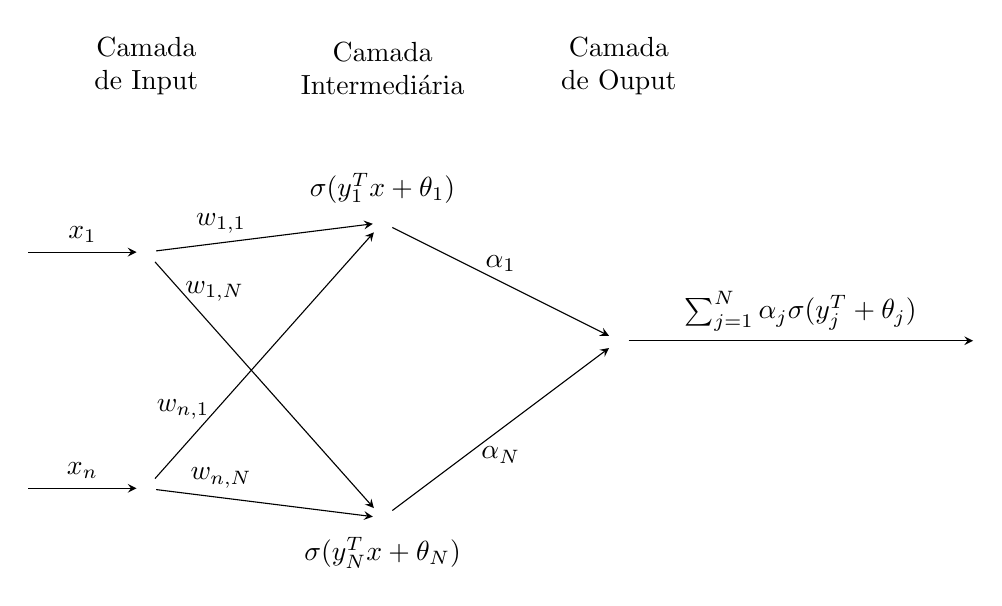
\begin{tikzpicture}[x=1.5cm, y=1.5cm, yshift=-1, >=stealth]

\foreach \m/\l [count=\y] in {1,missing,2}
  \node [every neuron/.try, neuron \m/.try] (input-\m) at (0,1.75-\y) {};

\foreach \m [count=\y] in {1,missing,2}
  \node [every neuron/.try, neuron \m/.try ] (hidden-\m) at (2,2.25-\y*1.25) {};

\foreach \m [count=\y] in {1}
  \node [every neuron/.try, neuron \m/.try ] (output-\m) at (4,1-\y) {};

\foreach \l [count=\i] in {1,n}
  \draw [<-] (input-\i) -- ++(-1,0)
    node [above, midway] {$x_\l$};

%% \foreach \l [count=\i] in {1,n}
%%   \node [above] at (hidden-\i.north) {$H_\l$};
\node [above] at (hidden-1.north) {\( \sigma (y_{ 1 }^{ T }x + \theta_{ 1 }) \)};
\node [below] at (hidden-2.south) {\( \sigma (y_{ N }^{ T }x + \theta_{ N }) \)};

\foreach \l [count=\i] in {1}
  \draw [->] (output-\i) -- ++(3,0)
    node [above, midway] {\( \sum_{ j=1 }^{ N } \alpha_{ j } \sigma (y_{ j }^{ T } + \theta_{ j }) \)};

%% \foreach \i in {1,...,2}
%%   \foreach \j in {1,...,2}
%%     \draw [->] (input-\i) -- (hidden-\j)
%%         node [above,pos=.2] {\( y_{ 1 }^{ (1) } \)};
\draw [->] (input-1) -- (hidden-1)
    node [above, pos=.3] {\( w_{ 1,1 } \)};
\draw [->] (input-2) -- (hidden-1)
    node [above, pos=.2, xshift=-2mm] {\( w_{ n,1 } \)};
\draw [->] (input-1) -- (hidden-2)
    node [above, pos=.2,xshift=2mm] {\( w_{ 1,N } \)};
\draw [->] (input-2) -- (hidden-2)
    node [above, pos=.3] {\( w_{ n,N } \)};

%% \foreach \i in {1,...,2}
%%   \foreach \j in {1}
%%     \draw [->] (hidden-\i) -- (output-\j);
\draw [->] (hidden-1) -- (output-1)
    node [above, midway] {\( \alpha_{ 1 } \)};
\draw [->] (hidden-2) -- (output-1)
    node [below, midway, yshift=-1mm] {\( \alpha_{ N } \)};

\foreach \l [count=\x from 0] in {de Input, Intermediária, de Ouput}
  \node [align=center, above] at (\x*2,2) {Camada \\ \l};

\end{tikzpicture}
    \end{center}
    \caption{Rede neural com apenas uma camada intermediária.
    Aqui temos \( x =
    \begin{bmatrix}
        x_{ 1 } & \cdots & x_{ n }
    \end{bmatrix}^{ T } \) e \( y_{ j }^{ T } =
    \begin{bmatrix}
        w_{ 1,j } & \cdots & w_{ n,j }
    \end{bmatrix} \), o vetor dos pesos de cada nó intermediário.
    Na última camada ocorre apenas uma combinação linear.}
    \label{fig: neural_net}
\end{figure}

A partir da segunda camada, cada nó está conectado a todos os nós da camada anterior por meio de uma aresta, a qual possui um peso.
Esse nó computa uma combinação linear, utilizando como coeficientes os pesos das arestas, dos valores armazenados pelos nós da camada anterior, soma um fator de correção ao valor obtido e passa o resultado por uma função não-linear, obtendo assim um valor próprio.
O caso em que \( m = 1 \) e há apenas uma camada intermediária de \( N \) nós, ao qual nos atentaremos, está representado na figura \ref{fig: neural_net}, onde \( \sigma \) é a não-linearidade.


Repare que o output da rede é exatamente a expressão em (\ref{eq: neural_func_form}).
Ou seja, o Teorema da Aproximação Universal, doravante conhecido como \uat , estabelece a possibilidade de aproximar arbitrariamente bem funções reais contínuas em \( \I^{ n } \) por meio de redes neurais com uma camada intermediária.
Essa é uma pergunta de extrema relevância, tanto teórica como prática pois, como apontado em \cite{lipmann}, redes neurais artificiais possuem diversas aplicações em campos voltados ao desenvolvimento de classificadores robustos, como a teoria de reconhecimento de fala e de imagens.
Saber que é possível realizar aproximações arbitrariamente boas utilizando redes neurais artificiais dá mais segurança e incentivo à pesquisa nessas áreas.

A demonstração do \uat \ envolve resultados de Teoria da Medida e Análise Funcional, os quais são importantes por si mesmos e, por isso, são discutidos em seções próprias.
Alguns conhecimentos necessários para entendê-los são apresentados como outro apêndice.
De fato, a demonstração desse resultado é mais densa que a dos outros, apesar de que ele, ao contrário do problema de Hilbert, lida apenas com aproximações.
Uma possível explicação para essa diferença será apresentada na seção correspondente.


% !TeX root = ./main.tex

\section{Teorema da aproximação de Weierstrass}

O primeiro teorema relacionado a aproximações de funções que estudaremos é o teorema da aproximação de Weierstrass, segundo o qual toda função contínua em um intervalo fechado pode ser bem proximada por um polinômio.
Inicialmente provado por Weierstrass em 1885, novas demonstrações surgiram com o tempo.
A que usamos de referência pode ser encontrada em \cite{weierstrass}.

Escolhemos começar com esse resultado por sua demonstração ser elementar, não exigindo mais que um curso de análise na reta.
Além disso, ele trata de aproximações em um contexto mais simples, envolvendo apenas uma variável, o que serve para acostumar o leitor ao tipo de questão que nos é de interesse.

Como dito anteriormente, desejamos mostrar que dada uma função contínua \( f : [a, b] \to \R \), podemos aproximá-la arbitrariamente bem por funções polinomiais \( p : [a, b] \to \R \).

Em outras palavras, seja \( C( [a, b]) \) o espaço vetorial das funções contínuas em \( [a, b] \). Indicamos por \( \norm{ \varphi }_{ \infty } \) a norma do supremo de uma função limitada \( \varphi : [a, b] \to \R \), ou seja, \[
    \norm{ \varphi }_{ \infty } = \sup \left\{ \abs{ \varphi(x) } \tq x \in [a, b] \right\}
.\]

Então é verdade que

\begin{teo}
    \label{thm: weierstrass}
    Dada \( f \in C( [a, b] ) \), para todo \( \varepsilon > 0 \) existe um polinômio \( p : [a, b] \to \R \) tal que \[
        \norm{ f - p }_{ \infty } < \varepsilon
    .\]
\end{teo}

Inicialmente, observamos que basta provar o teorema para o caso \( f \in C([0, 1]) \).
De fato, dada \( f \in C([a, b]) \), considere o homeomorfismo \( \varphi : [0, 1] \to [a, b] \) dado por \( \varphi(x) = a + ( b - a )x \), cuja inversa é \( \varphi^{ -1 } : [a, b] \to [0, 1] \) dada por \( \varphi^{ -1 } (x) = \frac{ x - a }{ b - a } \).
Então a função \( g = f \circ \varphi \) pertence a \( C([0, 1]) \) e, dado \( \varepsilon > 0 \), se existe um polinômio \( p(x) \) com \( \norm{ g - p }_{ \infty } < \varepsilon \), temos também, como \( \varphi^{ -1 } \) é um polinômio de grau \( 1 \), \[
    \norm{ g \circ \varphi^{ -1 } - p \circ \varphi^{ -1 } }_{ \infty } < \varepsilon
.\]
Como \( g \circ \varphi^{ -1 } = f \) e \( p \circ \varphi^{ -1 } \) é um polinômio, o resultado vale também para \( C([a, b]) \).

Em seguida, devemos definir a classe de polinômios que utilizaremos na demonstração.

\begin{defn}
    \label{def: bernstein}
    Dada \( g : \R \to \R \) definimos o \( n \)-ésimo polinômio de Bernstein de \( g \) como
    \begin{equation}
        B_{ n }(x, g) \defeq
        \sum_{ k=0 }^{ n } g \left( \frac{ k }{ n } \right) \binom{n}{k} x^{ k } ( 1 - x )^{ n - k }
        \label{eq: bernstein}
    .\end{equation}
\end{defn}

Note a semelhança entre os polinômios de Bernstein e a expansão binomial de \( ( 1 + ( 1 - x ) )^{ n } \).
De fato, temos \( B_{ n } (x, 1) = ( 1 + ( 1 - x ) )^{ n } = 1 \).
Mais geralmente, para toda constante \( c \in \R \) tem-se \( B_{ n } (x, c) = c \).

Utilizaremos essa semelhança para obter algumas identidades essenciais para a demonstração do teorema \ref{thm: weierstrass}.
Dados \( p \) e \( q \) reais, começamos considerando a expansão binomial de \( ( p + q )^{ n } \): \[
    ( p + q )^{ n } =
    \sum_{ k=0 }^{ n } \binom{n}{k} p^{ k } q^{ n-k }
.\]
Considerando ambos lados da igualdade como funções de \( p \), podemos derivá-los com relação a essa variável, obtendo \[
    n ( p + q )^{ n-1 } =
    \sum_{ k=0 }^{ n } k \binom{n}{k} p^{ k-1 } q^{ n-k }
.\]
Multiplicando ambos lados por \( p/n \), ficamos com
    \begin{equation}
        p ( p + q )^{ n-1 } =
        \sum_{ k=0 }^{ n } \frac{ k }{ n } \binom{n}{k} p^{ k } q^{ n-k }
        \label{eq: id_1}
    .\end{equation}
Essa é a primeira identidade, válida para todos \( p, q \in \R \).
Derivando novamente com relação a \( p \) e multiplicando ambos lados por \( p/n \) obtemos
\begin{equation}
    p^2 \left( 1 - \frac{ 1 }{ n } \right) ( p + q )^{ n-2 } + \frac{ p }{ n } ( p + q )^{ n-1 } =
    \sum_{ k=0 }^{ n } \frac{ k^2 }{ n^2 } \binom{n}{k} p^{ k } q^{ n-k }
    \label{eq: id_2}
,\end{equation}
a segunda identidade que utilizaremos.


Como consideramos \( f, g \in C([0, 1]) \), segue da Definição \ref{def: bernstein} que se \( f \geq 0 \), então \( B_{ n } (x, f) \geq 0 \) e, se \( f \leq g \), então \( B_{ n } (x, f) \leq B_{ n } (x, g) \).

Com essas ferramentas, podemos então apresentar a
 \begin{proof}[Demonstração do teorema \ref{thm: weierstrass}]
    Observamos inicialmente que como \( f \) é uma função contínua definida em um compacto, é uniformemente contínua.
    Portanto, dado \( \varepsilon > 0 \), existe \( \delta > 0 \) tal que, se \( x, y \in [0, 1] \) satisfazem \( \abs{ x - y } < \delta \), então \[
        \abs{ f(x) - f(y) } < \frac{ \varepsilon }{ 2 }
    .\]
    Agora, definimos \( M \defeq \norm{ f }_{ \infty } \) e fixamos \( \xi \in [0, 1] \).
    Logo, se \( \abs{ x - \xi } \geq \delta \) temos \[
        \abs{ f(x) - f(\xi) } \leq 2M \leq 2M \left( \frac{ x - \xi }{ \delta } \right)^2
    .\]
    Combinando as duas últimas desigualdades, concluímos que para todo \( x \in [0, 1] \) vale
    \begin{equation}
        \abs{ f(x) - f(\xi) } \leq 2M \left( \frac{ x - \xi }{ \delta } \right)^2 + \frac{ \varepsilon }{ 2 }
        \label{eq: weierstrass_bound_1}
    .\end{equation}

    Vamos aproximar \( f \) pelos seus polinômios de Bernstein.
    Seja \( B_{ n }(x, f) \) o \( n \)-ésimo polinômio de Bernstein de \( f \), avaliado em \( x \).
    Então
    \begin{align}
        \abs{ B_{ n } (x, f) - f(\xi) }
        &= \abs{B_{ n } (x, f - f(\xi))} \notag \\
        &\leq  B_{ n } \left( x, 2M \left( \frac{ x - \xi }{ \delta } \right)^2 + \frac{ \varepsilon }{ 2 } \right) \notag \\
        &= \frac{ 2M }{ \delta^2 } B_{ n } (x, ( x - \xi )^2) + \frac{ \varepsilon }{ 2 } \notag \\
        &+ \frac{ 2M }{ \delta^2 } \left( B_{ n } (x, x^2) + B_{ n } (x, -2 x \xi) + \xi^2 \right) + \frac{ \varepsilon }{ 2 } \notag \\
        &= \frac{ 2M }{ \delta^2 } \left( B_{ n } (x, x^2) - 2 \xi B_{ n } (x, x) + \xi^2 \right) + \frac{ \varepsilon }{ 2 }
        \label{al: elem_bernstein}
    .\end{align}
    Aqui fizemos uso das propriedades de \( B_{ n } (x, f) \) que seguem de \( x \in [0, 1] \), discutidas anteriormente.
    Utilizando as equações (\ref{eq: id_1}) e (\ref{eq: id_2}), com a substituição \( p = x \) e \( q = 1 - x \), concluímos que \[
        B_{ n } (x, x) = x
    .\]
    e que \[
        B_{ n } (x, x^2) = x^2 \left( 1 - \frac{ 1 }{ n } \right) + \frac{ x }{ n }
    .\]
    Substituindo em (\ref{al: elem_bernstein}), ficamos com
    \begin{align*}
        \frac{ 2M }{ \delta^2 } \left( B_{ n } (x, x^2) - 2 \xi B_{ n } (x, x) + \xi^2 \right) + \frac{ \varepsilon }{ 2 } &=
        \frac{ 2M }{ \delta^2 } \left( 
            x^2 \left( 1 - \frac{ 1 }{ n } \right) + \frac{ x }{ n }
            - 2 \xi x
            + \xi^2
         \right) + \frac{ \varepsilon }{ 2 } \\
         &= \frac{ 2M }{ \delta^2 } \left( 
             x^2 + \frac{ x - x^2 }{ n } - 2 \xi x + \xi^2
          \right) + \frac{ \varepsilon }{ 2 } \\
         &= \frac{ \varepsilon }{ 2 } + \frac{ 2M }{ n \delta^2 } ( x - x^2 ) + \frac{ 2M }{ \delta^2 } ( x - \xi )^2
    .\end{align*}
    Sendo assim, \[
        \abs{ B_{ n } (x, f) - f(\xi) } \leq \frac{ \varepsilon }{ 2 } + \frac{ 2M }{ n \delta^2 } ( x - x^2 ) + \frac{ 2M }{ \delta^2 } ( x - \xi )^2
    .\]
    Como essa desigualdade vale para todo \( x \in [0, 1] \), em especial é válida para \( x = \xi \).
    Fazendo essa substituição, obtemos \[
        \abs{ B_{ n } (\xi, f) - f(\xi) } \leq
        \frac{ \varepsilon }{ 2 } 
        + \frac{ 2M }{ n \delta^2 } ( \xi - \xi^2 )
    .\]
    Facilmente podemos verificar que \( \xi - \xi^2 \leq \frac{ 1 }{ 4 } \) para todo \( \xi \in [0, 1] \).
    Logo, \[
        \abs{ B_{ n } (\xi, f) - f(\xi) } \leq
        \frac{ \varepsilon }{ 2 } 
        + \frac{ M }{ 2 n \delta^2 }
    .\]
    Por fim, tomando \( n > \frac{ M }{ \varepsilon \delta^2 } \), temos \( \frac{ M }{ 2 n \delta^2 } < \frac{ \varepsilon }{ 2 } \) e, assim, \[
        \abs{ B_{ n } (\xi, f) - f(\xi) } < \varepsilon
    .\]
    Como o valor de \( n \) obtido para que essa desigualdade seja satisfeita depende apenas de \( \varepsilon \) (lembramos que \( \delta \) depende apenas de \( \varepsilon \), pela continuidade uniforme de \( f \)), ela é válida para todo \( \xi \in [0, 1] \), ou seja, \[
        \norm{ B_{ n } (\cdot , f) - f }_{ \infty } < \varepsilon
    .\qedhere\]
 \end{proof}
 


% !TeX root = ./main.tex
\section{Décimo Terceiro Problema de Hilbert}

Aqui provaremos a possibilidade de representar qualquer função contínua \( f : \I^{ n } \to \R \) por meio de composições e adições de funções contínuas de \( \R \to \R \) .
Com o trabalho de vários matemáticos, esse resultado foi generalizado.
Uma dessas generalizações é apresentada no teorema a seguir.

O leitor interassado poderá encontrar mais informações em \cite{hilbert}.
\begin{teo}[Kolmogorov, Arnol'd, Kahane, Lorentz e Sprecher]
    Para todo \( n \in \N \) com \( n \geq 2 \), existem números reais \( \lambda_{ 1 }, \lambda_{ 2 }, \dots, \lambda_{ n } \) e funções contínuas \( \varphi_{ k } : \I \to \R \), para \( k = 1, \dots, 2n + 1 \), com a propriedade de que para toda função contínua \( f : \I^{ n } \to \R \) existe uma função contínua \( g : \R \to \R \) tal que, para todo \( ( x_{ 1 }, \dots, x_{ n } ) \in \I^{ n } \),
    \begin{equation}
        f(x_{ 1 }, \dots, x_{ n }) =
        \sum_{ k=1 }^{ 2n+1 } g ( \lambda_{ 1 } \varphi_{ k } ( x_{ 1 } )  + \cdots + \lambda_{ n } \varphi_{ k } ( x_{ n } ) )
        \label{eq: kolmogorov_2}
    .\end{equation}
\end{teo}
\begin{rem}
    Denotamos o espaço das funções contínuas de \( \I^{ n } \) em \( \R \) por \( C(\I^{ n }) \).
    Notamos que esse espaço, com a norma do supremo, se torna um espaço métrico completo, com a distância dada por
    \begin{equation}
        d(f, g) = \norm{ f - g }_{ \infty }
    .\end{equation}
    O leitor pode encontrar resultados e definições elementares relativas a espaços métricos (inclusive o Teorema da Categoria de Baire, que será usado a seguir) no Apêndice \ref{ap: espacos_metricos}.
\end{rem}
Aqui nos atentaremos ao caso especial em que \( n = 2 \):
\begin{teo}
    Existem \( \lambda \in \R \backslash \Q \) e funções \( ( \varphi_{ 1 }, \dots, \varphi_{ 5 } ) \in [C(\I)]^{ 5 } \) tais que, para toda função \( f \in C(\I^{ 2 }) \) existe \( g : \R \to \R \), contínua, satisfazendo, para todos \( ( x_{ 1 }, x_{ 2 } ) \in \I^{ 2 } \), \[
        f ( x_{ 1 }, x_{ 2 } ) =
        \sum_{ k=1 }^{ 5 } g ( \varphi_{ k } ( x_{ 1 } ) + \lambda \varphi_{ k } ( x_{ 2 } ) )
    .\]
    \label{teo: hilbert13}
\end{teo}
\begin{rem}
    Por uma questão de economia de notação, definimos \[
        \Phi_{ k }(x, y) = \sum_{ k=1 }^{ 5 } \varphi_{ k } (x) + \lambda \varphi_{ k } (y)
    .\]
\end{rem}
Para a prova que apresentaremos, necessitamos de alguns lemas.
%% O primeiro deles clarifica a existência e a escolha de \( \lambda \).
%% \begin{lem}
%%     Existe um número real \( \lambda \) tal que, para quaisquer \( x_{ 1 }, x_{ 2 }, x_{ 3 }, x_{ 4 } \in \Q \), \[
%%         x_{ 1 } + \lambda y_{ 1 } = x_{ 2 } + \lambda y_{ 2 }
%%         \text{ implica }
%%         x_{ 1 } = x_{ 2 } \text{ e } y_{ 1 } = y_{ 2 }
%%     .\]
%%     \label{lem: lambda}
%% \end{lem}
%% \begin{proof}
%%     Basta escolher \( \lambda \in \R \backslash \Q \), pois se \( x_{ 1 } + \lambda y_{ 1 } = x_{ 2 } + \lambda x_{ 2 } \), então \( x_{ 1 } - x_{ 2 } = \lambda ( y_{ 2 } - y_{ 1 } ) \).
%%     Como \( x_{ 1 } - x_{ 2 } \in \Q \) necessariametente o lado direito deve ser \( 0 \), ou seja, \( y_{ 2 } = y_{ 1 } \) e \( x_{ 2 } = x_{ 1 } \).
%% \end{proof}
\begin{lem}
    Fixe \( \lambda \) irracional.
    Seja \( f \in C(\I^2) \) com \( \norm{ f }_{ \infty } = 1 \).
    Seja \( U_{ f } \) o suconjunto de \( [C(\I)]^{ 5 } \) tal que \( ( \varphi_{ 1 }, \dots, \varphi_{ 5 } ) \in U_{ f } \) se, e somente se, existe uma \( g \in C(\R) \) tal que
    \begin{equation}
        \abs{ g(t) } \leq \frac{ 1 }{ 7 } \text{ para todo } t \in \R
        \label{eq: g_bound}
    ,\end{equation}
    e
    \begin{equation}
        \abs{ 
            f(x, y)
            - \sum_{ i=1 }^{ 5 } (g \circ \Phi_{ k })(x, y) )
         }
         < \frac{ 7 }{ 8 }, \text{ para todo } x, y \in \I^2
         \label{eq: dif_bound}
    .\end{equation}
    Então \( U_{ f } \) é um suconjunto aberto e denso de \( [C(\I)]^{ 5 } \).
    \label{lem: uf}
\end{lem}
Enquanto é fácil perceber que \( U_{ f } \) é aberto, pois se \( \varphi = ( \varphi_{ 1 }, \dots, \varphi_{ 5 } ) \) satisfaz (\ref{eq: g_bound}) e (\ref{eq: dif_bound}) para uma dada \( g \), então todas as tuplas suficientemente perto de \( \varphi \) também satisfarão, a prova da densidade é mais extensa e será omitida, por não ser do interesse desse trabalho.
Nos restringimos a mencionar que ela necessita utiliza a hipótese da irracionalidade de \( \lambda \).
%% Colocar referência de onde ela pode ser encontrada
\begin{lem}
    Seja \( \lambda \) irracional.
    Então existem \( \varphi_{ 1 }, \dots, \varphi_{ 5 } \in C(\I) \) com a propriedade de que, dada \( f \in C(\I^2) \), existe uma \( g \in C(\R) \) satisfazendo \[
        \abs{ g(t) } \leq \frac{ 1 }{ 7 } \norm{ f }_{ \infty } \text{ para todo } t \in \R
    ,\]
    e \[
        \norm{ 
            f - \sum_{ k=1 }^{ 5 } g \circ \Phi_{ k }
         }_{ \infty } < \frac{ 8 }{ 9 } \norm{ f }_{ \infty }
    .\]
    \label{lem: baire}
\end{lem}
\begin{proof}
    Podemos supor, sem perda de generalidade, que \( \norm{ f }_{ \infty } = 1 \).
    Seja \( (h_{ j })_{ j\in\N } \) uma sequência de funções pertencentes a \( C(\I^2) \) tal que o conjunto \( \left\{ h_{ j } : j\in \N \right\} \) é denso na esfera unitária de \( C(\I^2) \).
    Na notação do Lema \ref{lem: uf}, cada \( h_{ j } \) determina um conjunto \( U_{ j } = U_{ h_{ j } } \subset  [C(\I)]^{ 5 } \) aberto e denso.
    Pelo Teorema da Categoria de Baire, o conjunto \[
        V = \bigcap_{ j\in\N } U_{ j }
    \]
    é denso em \( [C(\I)]^{ 5 } \).
    Pela densidade de \( \left\{ h_{ j } : j \in \N \right\} \), existe \( m \in \N \) tal que \( \norm{ f - h_{ m } }_{ \infty } < 1/72 \).
    Além disso, pelo Lema \ref{lem: uf} podemos tomar \( ( \varphi_{ 1 }, \dots, \varphi_{ 5 } ) \in V \subset  U_{ m } \) tal que exista \( g \in C(\I) \) satisfazendo \[
        \abs{ g(t) } \leq \frac{ 1 }{ 7 } \text{ para todo } t \in \R
    ,\]
    e \[
        \norm{ 
            h_{ m } - \sum_{ k=1 }^{ 5 } g \circ \Phi_{ k }
         }_{ \infty } < \frac{ 7 }{ 8 }
    .\]
    Com isso, \[
        \norm{ 
            f - \sum_{ k=1 }^{ 5 } g \circ \Phi_{ k }
         }_{ \infty } \leq
        \norm{ f - h_{ m } }_{ \infty }
        + \norm{ 
            h_{ m } - \sum_{ k=1 }^{ 5 } g \circ \Phi_{ k }
         }_{ \infty }
         < \frac{ 1 }{ 72 } + \frac{ 7 }{ 8 }
         = \frac{ 8 }{ 9 }
    ,\]
    o que termina a prova.
\end{proof}
Agora podemos enunciar a demonstração do Teorema \ref{teo: hilbert13}.
\begin{proof}[Demonstração do Teorema \ref{teo: hilbert13}]
    Pelo Lema \ref{lem: baire}, podemos fixar \( \lambda \in \R \) e \( \varphi_{ 1 }, \dots, \varphi_{ 5 } \in C(\I) \) tais que, dada \( f \in C(\I^2) \), existe \( g_{ 0 } \in C(\R) \) satisfazendo
    \begin{equation}
        \abs{ g_{ 0 }(t) } \leq \frac{ 1 }{ 7 } \norm{ f }_{ \infty } \text{ para todo } t \in \R
        \label{eq: g}
    ,\end{equation}
    e
    \begin{equation}
        \norm{ 
            f -
            \sum_{ k=1 }^{ 5 } g_{ 0 } \circ \Phi_{ k }
         }_{ \infty }
         < \frac{ 8 }{ 9 } \norm{ f }_{ \infty }
         \label{eq: f-(phi o g)}
    .\end{equation}
    Defina \( f_{ 0 } \defeq f \). Então, supondo definidas \( f_{ 0 }, \dots, f_{ n } \), \( g_{ 0 }, \dots, g_{ n } \), ponha \( f_{ n+1 } = f_{ n } - \sum_{ k=1 }^{ 5 } g_{ n } \circ \Phi_{ k } \).
    Logo, existe \( g_{ n+1 } \) satisfazendo (\ref{eq: g}) e (\ref{eq: f-(phi o g)}) com \( g_{ n+1 } \) no lugar de \( g_{ 0 } \) e \( f_{ n+1 } \) no lugar de \( f \).
    
    Dessa forma, temos \( \norm{ g_{ n } }_{ \infty } \leq \frac{ 1 }{ 7 } \norm{ f_{ n } }_{ \infty } \) e \( \norm{ f_{ n+1 } }_{ \infty } = \norm{ f_{ n } - \sum_{ k=1 }^{ 5 } g_{ n } \circ \Phi_{ k } }_{ \infty } \leq \frac{ 8 }{ 9 } \norm{ f_{ n } }_{ \infty } \).
    Portanto, \[
        \norm{ f_{ n } }_{ \infty } \leq \left( \frac{ 8 }{ 9 } \right)^{ n } \norm{ f_{ 0 } }_{ \infty } = \left( \frac{ 8 }{ 9 } \right)^{ n } \norm{ f }_{ \infty }
    ,\]
    e \[
        \norm{ g_{ n } }_{ \infty } <
        \frac{ 1 }{ 7 } \left( \frac{ 8 }{ 9 } \right)^{ n } \norm{ f }
    .\]
    Sendo assim, a série \( \sum g_{ n } \) absolutamente para uma certa \( g \in C(\R) \) e, com isso, \[
        f = \sum_{ n\in\N } f_{ n } - f_{ n+1 }
        = \sum_{ n\in\N } \sum_{ k=1 }^{ 5 } g_{ n } \circ \Phi_{ k }
        = \sum_{ k=1 }^{ n } \left( 
            \sum_{ n\in\N } g_{ n }
         \right)
         \circ \Phi_{ k }
        = \sum_{ k=1 }^{ 5 } g \circ \Phi_{ k }
    ,\]
    o que conclui a demonstração.
\end{proof}

% !TeX root = ./main.tex
\section{Teorema de Hahn-Banach}

Se \( V \) é um espaço vetorial real, um \emph{funcional sublinear} em \( V \) é uma função \( p : V \to \R \) tal que
\begin{equation}
    p ( x + y ) \leq p(x) + p(y) \text{ e } p(\lambda x) = \lambda p(x) \text{ para todos \( x, y \in V \) e \( \lambda \in \R_{ \geq 0 } \)}
.\end{equation}
Observe que nada se exige sobre o sinal de \( p \).
Um exemplo de funcional sublinear é uma seminorma em \( V \).

\begin{teo}[Hahn-Banach]
    \label{thm: hahn-banach}
    Sejam \( V \) um espaço vetorial real, \( M \) um subespaço de \( V \) e \( p \) um funcional sublinear em \( V \).
    Se \( f \) é um funcional linear em \( M \) dominado por \( p \), ou seja, tal que \( f(v) \leq p(v) \) para todo \( v \in M \), então existe um funcional linear \( F \) em \( V \), que coincide com \( f \) em \( M \) e que também é dominado por \( p \).
    O funcional \( F \) é dito \emph{extensão de Hahn-Banach} de \( f \).
\end{teo}

Em outras palavras, se, em um espaço vetorial, temos um funcional sublinear que domina um funcional linear definido em um subespaço, podemos extender esse funcional ao espaço todo, mantendo a relação de dominância.

Antes de apresentar a demonstração do teorema \ref{thm: hahn-banach}, vamos introduzir alguns conceitos de Teoria dos Conjuntos.

%% Escrever sobre o teorema, dar uma intuição da importância dele

\subsection{Lema de Zorn}

Dados conjuntos \( X \) uma \emph{relação} de \( X \) em \( Y \) é um subconjunto \( R \) de \( X \times Y \). 
Escreveremos \( x R y \) para indicar que \( ( x, y ) \in R \).
Perceba que uma função \( f : X \to Y \) é uma relação de \( X \) em \( Y \) dada por \( ( x, y ) \in f \) se, e somente se, \( y = f(x) \).
Quando \( R \subset X \times X \), diremos que \( R \) é uma relação em \( X \).

Uma \emph{relação de ordem parcial} em \( X \) é uma relação que satisfaz, dados \( x, y, z \in X \):
\begin{enumerate}[label=\roman*)]
    \item \( x R x \) (\emph{reflexividade});
    \item Se \( x R y \) e \( y R x \), então \( x = y \) (\emph{antisimetria});
    \item Se \( x R y \) e \( y R z \), então \( x R z \) (\emph{transitividade}).
\end{enumerate}
O termo \emph{parcial} é utilizado para indicar que podem existir elementos de \( X \) não relacionados por essa ordem.
Caso tenhamos \( x R y \) ou \( y R x \) para todos \( x, y \in X \), então \( R \) é dita uma relação de ordem \emph{total}.
Utilizaremos o símbolo \( \prec \) para indicar uma ordem parcial.
Dizemos então que \( ( X, \prec ) \) é um conjunto parcialmente ordenado.
Se \( \prec \) também é total, \( ( X, \prec ) \) é totalmente ordenado.
Claramente todo subconjunto de \( X \) também é parcialmente ordenado, com a ordem induzida por \( \prec \).

Um \emph{elemento maximal} de um conjunto ordenado \( X \) é um elemento \( x \) tal que se \( y \in X \) com \( x \prec y \), então \( y = x \).
Uma \emph{cota superior} de um subconjunto \( Y \subset X \) é um elemento \( x \in X \) tal que \( y \prec x \) para todo \( y \in Y \).
Observe que se \( \prec \) não é total, não necessariamente um elemento maximal de \( Y \subset X \) é uma cota superior de \( Y \).

Dois exemplos usuais de conjuntos ordenados são \( \R \) e \( \mathcal{P} ( X ) \), para um dado conjunto \( X \).
O primeiro é um conjunto totalmente ordenado pela ordem usual \( \leq \), o qual não possui elemento maximal.
O segundo se torna um conjunto ordenado ao dizermos que dados \( A, B \subset X \), temos \( A \prec B \) se, e somente se \( A \subset  B \).
Essa ordem não é total e o único elemento maximal de \( \mathcal{P} ( X ) \) é o próprio \( X \).

\begin{axiom}[lema de Zorn]
    Todo conjunto parcialmente ordenado, tal que todos seus subconjuntos totalmente ordenados possuam cota superior, possui elemento maximal.
\end{axiom}

Encerramos essa apresentação com um resultado que exemplifica como o lema de Zorn geralmente é utilizado.

\begin{prop}
    Todo espaço vetorial não trivial, ou seja, que possui elementos não nulos, possui uma base.
\end{prop}
\begin{proof}
    Seja \( V \) o espaço vetorial em questão, e \( A \) a coleção de todos os subconjuntos linearmente independentes de \( V \).
    Claramente essa coleção é parcialmente ordenada pela relação de inclusão.
    Dada uma subcoleção \( B \subset A \) totalmente ordenada, considere o conjunto
    \begin{equation}
        C = \bigcup_{ \beta \in B } \beta
    .\end{equation}
    Afirmamos que \( C \in A \).
    De fato, dado um conjunto finito \( \left\{ x_{ 1 }, \dots, x_{ n } \right\} \subset C \), sejam \( \beta_{ 1 }, \dots, \beta_{ n } \) os conjuntos de \( B \) tais que \( x_{ i } \in \beta_{ i } \) para todo \( i \leq n \).
    Como \( B \) é totalmente ordenado, existe \( \beta_{ k } \) tal que \( \beta_{ i } \subset \beta_{ k } \) para todo \( i \leq n \).
    Logo \( \left\{ x_{ i }, \dots, x_{ n } \right\} \subset  \beta_{ k } \) e, como \( \beta_{ k } \) é linearmente independente, também o são os \( x_{ i } \).
    Dessa forma, \( C \) é um conjunto linearmente independente, pertencente a \( A \) e que claramente é uma cota superior de \( B \).

    Portanto, aplicando o lema de Zorn obtemos um elemento maximal \( \Lambda \) de \( A \).
    Denotando por \( \lin \Lambda \) o conjunto formado pelas combinações lineares de elementos de \( \Lambda \), afirmamos que \( \lin \Lambda = A \).
    Com efeito, supondo, por absurdo, que exista \( v \in V \backslash \lin \Lambda \), temos que \( \Lambda \cup \left\{ v \right\} \) é linearmente independente, ou seja, pertence a \( A \) e contém \( \Lambda \), um contradição pois \( \Lambda \) é maximal.
\end{proof}

\subsection{Demonstração do teorema de Hahn-Banach}

Seja \( \left\{ g_{ \lambda } \right\}_{ \lambda \in L } \), para algum conjunto de índices \( L \), a coleção das extensões lineares de \( f \) em conjuntos \( M_{ \lambda } \) tais que \( M \subset  M_{ \lambda } \subset V \), que são dominadas por \( p \).
Como \( f \in \left\{ g_{ \lambda } \right\}_{ \lambda \in L } \), essa coleção é não-vazia e, portanto, podemos ordená-la parcialmente utilizando a relação de inclusão, considerando que \( g_{ \lambda } \) é um subconjunto de \( M_{ \lambda } \times \R \).
Mais especificamente, diremos que \( g_{ \alpha } \subset g_{ \beta } \) se tivermos \( M_{ \alpha } \subset M_{ \beta } \) e \( g_{ \beta } \mid_{ M_{ \alpha } } = g_{ \alpha } \), ou seja, se \( g_{ \beta } \) for uma extensão de \( g_{ \alpha } \).
Desejamos mostrar que existe um elemento maximal de \( \left\{ g_{ \lambda } \right\}_{ \lambda \in L } \).
Dado \( L' \subset L \) tal que \( \left\{ g_{ \lambda } \right\}_{ \lambda \in L' } \) é uma subcoleção totalmente ordenada, definimos \( g \) como
\begin{equation}
    g \defeq \bigcup_{ \lambda \in L' } g_{ \lambda }
,\end{equation}
ou seja, \( g \) é um funcional linear em \( \bigcup_{ \lambda \in L } M_{ \lambda } \) tal que \( g(v) = g_{ \lambda } (v) \), onde \( v \in M_{ \lambda } \).
De fato \( g \) está bem definida, pois se \( v \in M_{ \lambda_{ 1 } } \cap M_{ \lambda_{ 2 } } \) com \( \lambda_{ 1 } \neq \lambda_{ 2 } \), ambos pertencentes a \( L' \), então podemos supor, sem perda de generalidade, que \( g_{ \lambda_{ 2 } } \subset g_{ \lambda_{ 1 } } \) e, assim, \( g_{ \lambda_{ 1 } } (v) = g_{ \lambda_{ 2 } }(v) \), para \( v \in M_{ \lambda_{ 1 } } \cap M_{ \lambda_{ 2 } } = M_{ \lambda_{ 2 } } \). 
É fácil verificar que \( g \) estende \( f \) e é dominado por \( p \).
Logo, \( g \) é uma cota superior de \( \left\{ g_{ \lambda } \right\}_{ \lambda \in L' } \) e, pelo lema de Zorn, existe \( F \in \left\{ g_{ \lambda } \right\}_{ \lambda \in L } \), definido em \( W \subset  V \), maximal.

Intuitivamente é claro que \( F \) deve estar definida em todo o espaço \( V \), de modo que é a extensão de Hahn-Banach de \( f \).
Para demonstrar esse fato, suponha, por absurdo, que ele seja falso, ou seja, que exista \( \eta \in V \backslash W \).
Nossa estratégia será construir um uma extensão \( G \) de \( F \), dominada por \( p \), definida em \( U = \lin (W \cup \left\{ \eta \right\}) \), contradizendo a maximalidade de \( F \).

Para definirmos \( G \), basta atribuirmos um valor para \( G(\eta) \).
De fato, todo elemento de \( U \) é da forma \( w + \alpha \eta \), onde \( w \in W \) e \( \alpha \in \R \).
Logo, pondo
\begin{equation}
    G(w + \alpha \eta) = F(w) + \alpha G(\eta)
,\end{equation}
claramente \( G \) é uma extensão de \( F \).
O passo crucial é definir \( G(\eta) \) de forma que \( G \) seja dominada por \( p \).
Para tanto, vamos nos atentar a algumas desigualdades.
Dados \( w_{ 1 }, w_{ 2 } \in W \), vale
\begin{equation}
    F(w_{ 1 }) + F(w_{ 2 }) =
    F(w_{ 1 } + w_{ 2 }) \leq
    p(w_{ 1 } + w_{ 2 }) \leq
    p(w_{ 1 } - \eta) + p(\eta + w_{ 2 })
.\end{equation}
Equivalentemente:
\begin{equation}
    F(w_{ 1 }) - p(w_{ 1 } - \eta) \leq p(\eta + w_{ 2 }) - F(w_{ 2 })
.\end{equation}
Ou seja, temos
\begin{equation}
    \sup \left\{ F(w_{ 1 }) - p(w_{ 1 } - \eta) \tq w_{ 1 } \in W \right\} \leq
    \inf \left\{ p(\eta + w_{ 2 }) - F(w_{ 2 }) \tq w_{ 2 } \in W \right\}
.\end{equation}
Defina, então, \( G(\eta) \) de modo que
\begin{equation}
    \sup \left\{ F(w_{ 1 }) - p(w_{ 1 } - \eta) \tq w_{ 1 } \in W \right\} \leq
    G(\eta) \leq
    \inf \left\{ p(\eta + w_{ 2 }) - F(w_{ 2 }) \tq w_{ 2 } \in W \right\}
.\end{equation}
Dessa forma, dado \( w + \alpha \eta \in U \), se \( \alpha > 0 \) temos
\begin{align}
    G(w + \alpha \eta) &=
    F(w) + \alpha G(\eta) \\
    &\leq F(w) + \alpha \left( 
        p \left( \frac{ w }{ \alpha } + \eta \right) - F \left(  \frac{ w }{ \alpha }  \right)
    \right) \\
    &= F(w) + p(w + \alpha \eta) - F(w) \\
    &= p(w + \alpha \eta)
.\end{align}
Caso \( \alpha < 0 \):
\begin{align}
    G(w + \alpha \eta) &=
    F(w) + \alpha G(\eta) \\
    &\leq F(w) + \alpha \left( 
        F \left( \frac{ w }{ \abs{ \alpha } } \right) -
        p \left( \frac{ w }{ \abs{ \alpha } } - \eta \right)
    \right) \\
    &= F(w) - F(w) - p(-w - \alpha \eta) \\
    &= p(w + \alpha \eta)
.\end{align}
Se \( \alpha = 0 \), \( G \) coincide com \( F \) e claramente é dominada por \( p \).
Sendo assim, chegamos a uma contradição com a maximalidade de \( F \), o que conclui a prova. \qed

No caso especial em que \( p \) é uma seminorma, a condição \( f \leq p \) é equivalente a \( \abs{ f } \leq p \), pois \( -f(x) = f(-x) \leq p(-x) = p(x) \).

\subsection{Aplicações do teorema de Hahn-Banach}

Aqui vamos utilizar o teorema de Hahn-Banach para provar um resultado sobre subespaços vetoriais densos que será utilizado na prova do teorema da Aproximação Universal.
Começamos apresentando uma aplicação do teorema de Hahn-Banach para ilustrar como ele é geralmente utilizado.

\begin{teo}
    Seja \( V \) um espaço vetorial normado.
    Então:
    \begin{enumerate}[label=\roman*)]
        \item Se \( 0 \neq v \in V \), então existe \( f \in V^{ * } \) tal que \( f(v) = \norm{ v } \) e \( \norm{ f } = 1 \);
        \item Se \( v \) e \( w \) são elementos distintos de \( V \), então existe \( f \in V^{ * } \) tal que \( f(v) \neq f(w) \);
        \item Se \( v \in V \) satisfaz \( f(v) = 0 \) para todo \( f \in V^{ * } \), então \( v = 0 \);
        \item Se \( v \in V \), então
        \begin{equation}
            \norm{ v }
            = \sup_{ 0 \neq f \in V^{ * } } \frac{ \abs{ f(v) } }{ \norm{ f } }
            = \max_{ 0 \neq f \in V^{ * } } \frac{ \abs{ f(v) } }{ \norm{ f } }
        .\end{equation}
    \end{enumerate}
\end{teo}
\begin{proof}
    Para provar \emph{i}, basta aplicar Hahn-Banach com o funcional sublinear dado pela norma, o subespaço \( M = \lin (\left\{ v \right\}) \) e o funcional \( f : M \to \R \) dado por \( f(\alpha v) = \alpha \norm{ v } \).
    Sendo \( F \) a extensão de Hahn-Banach de \( f \), temos \( F(v) = \norm{ v } \) e, como o funcional sublinear é a norma de \( V \), vale \( \abs{ F(x) } \leq \norm{ x } \) para todo \( x \in V \).
    Como há um caso de igualdade, vale \( \norm{ F } = 1 \).
    Em \emph{ii}, como \( v \neq w \), então \( v - w \neq 0 \).
    Por \emph{i}, isso implica a existência de um funcional \( f \) tal que \( f(v - w) = \norm{ v - w } \neq 0 \), ou seja, \( f(v) \neq f(w) \).
    Claramente \emph{iii} segue diretamente de \emph{ii}.
    Como, para todo \( f \in V^{ * } \), vale \( \abs{ f(v) } \leq \norm{ f } \norm{ v } \), temos
    \begin{equation}
        \norm{ v } \geq \sup_{ 0 \neq f \in V^{ * } } \frac{ \abs{ f(v) } }{ \norm{ f } }
    .\end{equation}
    Por \emph{i}, existe \( g \in V^{ * } \) tal que \( g(v) = \norm{ v } \) e \( \norm{ g } = 1 \), de modo que
    \begin{equation}
        \norm{ v } = \frac{ \abs{ g(v) } }{ \norm{ g } }
    ,\end{equation}
    ou seja, vale a igualdade e podemos trocar \( \sup \) por \( \max \).
\end{proof}

A próxima proposição será útil para provar o principal resultado dessa seção.
\begin{prop}
    Seja \( V \) um espaço vetorial normado e \( M \) um subespaço próprio fechado de \( V \).
    Dado \( v \in V \backslash M \), definimos \( \delta = d(v, M) \defeq \inf \left\{ \norm{ v - w } : w \in M \right\} \).
    Então existe um funcional \( f \in V^{ * } \) tal que \( \norm{ f } = 1 \), \( f(v) = \delta \) e \( f  \mid_{ M } = 0 \).
    \label{prop: closed_subset}
\end{prop}
\begin{proof}
    Como \( M \) é fechado, \( \delta > 0 \).
    Defina o funcional \( g : \lin ( \left\{ v \right\} \cup M ) \to \R \) dado por
    \begin{equation}
        g(\alpha v + w) = \alpha \delta
    ,\end{equation}
    onde \( \alpha \in \R \) e \( w \in M \).
    Claramente temos \( g \mid_{ M } = 0 \) e \( g(v) = \delta \).
    Agora perceba que
    \begin{equation}
        \abs{ g(\alpha v + w) } = \abs{ \alpha } \delta \leq \abs{ \alpha } \norm{ v + w / \alpha } = \norm{ \alpha v + w }
    ,\end{equation}
    de modo que \( \norm{ g } \leq 1 \).
    Além disso, para todo \( w \in M \) vale
    \begin{equation}
        \norm{ g } \geq \frac{ \abs{ g(v + w) } }{ \norm{ v + w } } = \frac{ \delta }{ \norm{ v + w } }
    .\end{equation}
    Portanto,
    \begin{equation}
        \norm{ g } \geq \sup_{ w \in M } \frac{ \delta }{ \norm{ v + w } } = \frac{ \delta }{ \inf_{ w \in M } \norm{ v - w } } = 1
    .\end{equation}
    Logo, \( \norm{ g } \geq 1 \) e, com isso, \( \norm{ g } = 1 \).
    Agora podemos aplicar Hahn-Banach, obtendo a extensão \( f \) de \( g \), utilizando como funcional sublinear a norma em \( V \).
\end{proof}

Agora o teorema que será usada na prova do teorema da Aproximação Universal.

\begin{teo}
    Um subespaço \( M \) de um espaço vetorial \( V \) é denso se, e somente se, o único elemento de \( V^{ * } \) que se anula em \( M \) é o funcional nulo.
\end{teo}
\begin{proof}
    Suponha que \( N \) é um subespaço denso de \( V \) e seja \( f \in V^{ * } \) um funcional que se anula em \( M \).
    Dado \( v \in V \backslash M \), seja \( ( x_{ n } )_{ n \in \N } \) tal que \( x_{ n } \in M \) para todo \( n \) e \( x_{ n } \to v \).
    Como \( f \) é uma transformação linear limitada, é contínua e, portanto, \( f(x_{ n }) \to f(v) \).
    Porém \( f(x_{ n }) = 0 \) para todo \( n \), ou seja, \( f(x_{ n }) \to 0 = f(v) \), de modo que \( f = 0 \).

    Reciprocamente, se o único elemento de \( V^{ * } \) que se anula em \( M \) é o funcional nulo, então necessariamente \( V \) é denso.
    Caso contrário, \( \overline{M} \) seria um subespaço próprio fechado de \( V \) e, pela proposição \ref{prop: closed_subset} existiria um funcional não nulo que se anula em \( \overline{M} \) e, consequentemente, em \( M \).
\end{proof}
\section{Teorema da Representação de Riesz}

Esse teorema possui diversas formulações.
Em geral, elas têm como objetivo representar os funcionais lineares contínuos em um dado espaço vetorial de uma maneira mais natural, associando-os a elementos daquele mesmo espaço ou de outro, por meio de um produto interno ou uma operação semelhante.

Apesar de a versão que abordaremos inicialmente não ser a utilizada na demonstração do \uat, acreditamos que é importante apresentar esse teorema primeiro no contexto natural de espaços de Hilbert.

Novamente, nossa exposição desse resultado clássico da Análise Funcional foi formulada com base em \cite{func-anal} e o leitor que quiser recordar conceitos fundamentais poderá encontrálos no Apêndice \ref{app: func anal}.

\subsection{Em espaços de Hilbert}

Da forma que será primeiramente enunciado, esse resultado trata da associação natural que existe entre um espaço de Hilbert \( H \) e o seu dual, \( H^{ * } \). Apesar de ser um fato de certa forma trivial para espaços de dimensão finita, sua demonstração não é tão óbvia para espaços de Hilbert em geral.
Para demonstrá-lo, precisamos, antes, de passar por três resultados preliminares.

\begin{lem}
    Dados \( v, w \) pertencentes a \( (V, \dotprod{\cdot,\cdot}) \), tem-se que \( v \perp w \), ou seja, \( \dotprod{v,w} = 0 \), se, e somente se,
    \begin{equation}
        \norm{ v + \lambda w } \geq \norm{ v }
        \label{eq: ineq}
    .\end{equation}
    para todo \( \lambda \in \R \).
    \label{lem: perp_equiv}
\end{lem}
\begin{proof}
    Evidementemente temos \[
        0
        \leq \norm{ v + \lambda w }^2
        = \norm{ v }^2 + 2 \Re (\dotprod{v,w}) + \abs{ \lambda }^2 \norm{ w }^2
    .\]
    Se \( v \perp w \), então temos
    \begin{align*}
        \norm{ v + \lambda w }^2
        &= \norm{ v }^2 + \abs{ \lambda }^2 \norm{ w }^2 \\
        &\geq \norm{ v }^2
    ,\end{align*}
    de onde a desigualdade (\ref{eq: ineq}) segue.
    Reciprocamente, se vale (\ref{eq: ineq}) para todo \( \lambda \in \K \), em especial tomando \( \lambda = -\dotprod{w,v}/ \norm{ w }^2 \) e elevando ambos lados ao quadrado ficamos com \( 0 \leq - \abs{ \dotprod{v,w} }^2 \), o que implica \( v \perp w \).
\end{proof}

\begin{lem}[Lei do paralelogramo]
    Dados \( v, w \) pertencentes a \( (V, \dotprod{\cdot,\cdot}) \), tem-se \[
        \norm{ v + w }^2 + \norm{ v - w }^2 = 2 \norm{ v }^2 + 2 \norm{ w }^2
    .\]
\end{lem}

Como a demonstração desse lema consiste simplesmente em expandir o lado esquerdo da igualdade e usar as propridedades de produto interno, será deixada a cargo do leitor.

Antes do próximo resultado, uma definição.
Dado um subespaço \( E \) de um espaço com produto interno \( V \), definimos \[
    E^{ \perp } = \left\{ v \in V : \dotprod{v,w} = 0 \text{ para todo } w \in E \right\}
.\]

\begin{teo}[Projeção ortogonal]
    \label{teo: proj_ort}
    Se \( E \) é subespaço vetorial fechado de um espaço de Hilbert \( H \), então \[
        H = E \oplus E^{ \perp }
    .\]
\end{teo}
\begin{proof}
    Dado \( v \in H \), definimos \( \delta = \inf \left\{ \norm{ v - w } : w \in E \right\} \).
    Seja \( (w_{ n })_{ n\in\N } \) uma sequência de elementos de \( E \) tais que \( \norm{ v - w_{ n } } \to \delta \).
    Então, sendo \( k \) e \( \ell \) números naturais, aplicando a lei do paralelogramo para os vetores \( w_{ k } - v \) e \( w_{ \ell } - v \) obtemos: \[
        2 \norm{ w_{ k } - v }^2 + 2 \norm{ w_{ \ell } - v }^2
        = \norm{ w_{ k } + w_{ \ell } - 2v }^2 + \norm{ w_{ k } - w_{ \ell } }
    ,\]
    o que implica, remanejando e lembrando que \( (w_{ k } + w_{ \ell })/2 \in E \),
    \begin{align*}
        \norm{ w_{ k } - w_{ \ell } }
        &= 2 \norm{ w_{ k } - v }^2 + 2 \norm{ w_{ \ell } - v }^2 - 4 \norm{ (w_{ k } + w_{ \ell })/2 - v }^2 \\
        &\leq 2 \norm{ w_{ k } - v }^2 + 2 \norm{ w_{ \ell } - v }^2 - 4 \delta^2
    .\end{align*}
    Com isso, concluímos que \( (w_{ n }) \) é uma sequência de Cauchy.
    Como \( H \) é um espaço de Hilbert, temos que \( w_{ n } \to w \in E \), pois \( E \) é fechado e, pela continuidade da norma, temos \( \norm{ v - w } = \delta \).

    Intuitivamente, \( w \) é o elemento de \( E \) mais próximo de \( v \).
    Logo, é razoável esperar que ele seja a projeção ortogonal de \( v \) em \( E \).
    Para confirmar essa suspeita, devemos verificar que \( v - w \in E^{ \perp } \).
    De fato, para todo \( \lambda \in \K \) e todo \( u \in E \) temos \[
        \norm{ (v - w) + \lambda u }
        = \norm{ v + (-w + \lambda u) }
        \geq \delta
        = \norm{ v - w }
    .\]
    Portanto, pelo Lema \ref{lem: perp_equiv}, concluímos que \( v - w \in E^{ \perp } \).
    Sendo assim, temos \( v = w + (v - w) \), onde \( w \in E \) e \( v - w \in E^{ \perp } \).
    Para mostrar a unicidade dessa decomposição, suponha que \( v = w_{ 1 } + u_{ 1 } = w_{ 2 } + u_{ 2 } \), onde \( w_{ 1 }, w_{ 2 } \in E \) e \( u_{ 1 }, u_{ 2 } \in E^{ \perp } \).
    Então \[
        w_{ 1 } - w_{ 2 } = u_{ 2 } - u_{ 1 } \in E \cap E^{ \perp }
    ,\]
    o que implica \( w_{ 1 } - w_{ 2 } = u_{ 2 } - u_{ 1 } = 0 \), ou seja, \( w_{ 1 } = w_{ 2 } \) e \( u_{ 1 } = u_{ 2 } \).
\end{proof}

Agora podemos prosseguir para o principal resultado dessa subseção.

\begin{teo}[Teorema da representação de Riesz em espaços de Hilbert]
    Dado um espaço de Hilbert H e seu dual \( H^{ * } \), a função
    \begin{align*}
        \gamma : &H \to H^{ * } \\
            &v \mapsto \gamma(v) = f_{ v }
    ,\end{align*}
    tal que \( f_{ v } = \dotprod{v,\cdot} \), é uma isometria antilinear e sobrejetiva em \( H^{ * } \).
\end{teo}
    Repare que, devido à sobrejetividade, todo funcional \( f \in H^{ * } \) fica unicamente associado a um determinado \( v \in H \) tal que \( f = \gamma(v) \).
    Dizemos, então, que \( v \) \emph{representa} \( f \).
\begin{proof}
    Para mostrar que \( \gamma \) é uma isometria, provaremos que \( \norm{ f_{ v } } = \norm{ v } \) para todo \( v \in H \).
    De fato, se \( v = 0 \) isso é evidente.
    Fixado \( v \in H \backslash \left\{ 0 \right\} \), pela desigualdade de Cauchy-Schwarz temos \( \abs{ f_{ v }(w) } = \abs{ \dotprod{v,w} } \leq \norm{ v } \norm{ w } \).
    Logo, \( \norm{ f_{ v } } \leq \norm{ v } \).
    Por outro lado, temos \( \norm{ v }^2 = \dotprod{v,v} = f_{ v }(v) \leq \norm{ f_{ v } } \norm{ v } \), ou seja, \( \norm{ v } \leq \norm{ f_{ v } } \) e acabamos.

    Além disso claramente \( \gamma \) é antilinear, pois \[
        \gamma (\alpha v + w) = \dotprod{\alpha v + w, \cdot} = \bar{\alpha} \dotprod{v, \cdot} + \dotprod{w,\cdot} = \bar{\alpha} \gamma(v) + \gamma(w)
    .\]

    A parte menos óbvia, e que dá nome ao teorema, é a da sobrejetividade.
    Para demonstrá-la, utilizaremos o Teorema \ref{teo: proj_ort}.

    Dado \( f \in H^{ * } \), se \( f = 0 \) então naturalmente \( f = \gamma(0) \).
    Se \( f \neq 0 \), repare que \( \ker(f) \), o núcleo de \( f \), é um subespaço próprio fechado de \( H \).
    Pelo Teorema \ref{teo: proj_ort}, temos \[
        H = \ker(f) \oplus \ker(f)^{ \perp }
    ,\]
    de onde concluímos que existe \( w \in \ker(f)^{ \perp } \) satisfazendo \( \norm{ w } = 1 \).
    Agora uma observação simples, porém fundamental: para todos \( u, v \in H \) temos \( f(v)u - f(u)v \in \ker(f) \).
    Logo, para todo \( v \in H \) temos \[
        \dotprod{w,f(v)w - f(w)v} = 0
    ,\]
    o que implica, desenvolvendo, \[
        f(v) = \dotprod{\overline{f(w)}w,v}
    .\]
    Sendo assim, \( f = \gamma(\overline{f(w)}w) \).
\end{proof}

\subsection{Em Teoria da Medida}

No contexto de teoria da medida, existem alguns resultados que são reconhecidos como ``teorema da representação de Riesz''.
O mais conhecido estabelece que dual do espaço das funções cujo módulo é \( p \) integrável em um espaço de medida \( (\Omega, \Sigma, \mu) \), denominado espaço \( L_{ p } \), onde \( 1 < p < +\infty \), é representado pelo espaço \( L_{ q } \), onde \( 1/p + 1/q = 1 \).
Mais precisamente, se \( G : L_{ p } \to \R \) é um funcional linear limitado, então existe \( g \in L_{ q } \) tal que, para toda \( f \in L_{ p } \) temos \[
    G(f) = \int fg \ \mathrm{d}\mu
.\]
Se \( \mu \) é uma medida \( \sigma \)-finita, então o resultado também é válido para \( L_{ 1 } \), cujo espaço dual é \( L_{ \infty } \).
Observe que se \(  p = q = 2 \), então o espaço \( L_{ 2 } \) é um espaço de Hilbert e, então, o teorema da representação de Riesz se torna o mesmo apresentado na subseção anterior.

Outro teorema que também leva esse nome, e que é o que utilizaremos para provar o \uat, utiliza medidas para representar funcionais definidos num espaço de funções reais contínuas.
A versão exata de que precisamos tem uma demonstração que foge do escopo deste trabalho, portanto, antes de apresentá-la vamos enunciar e demonstrar uma versão mais simples, que trata dos funcionais definidos em \( C([a, b]) \).
Porém antes, uma definição:
\begin{defn}
    Dado um espaço \( \mathcal{F} \) formado pelas funções de um conjunto qualquer \( X \) em \( \R \), um funcional linear \( G : \mathcal{F} \to \R \) é dito \emph{positivo} se \( G(f) \geq 0 \) sempre que \( f \geq 0 \), ou seja, sempre que \( f(x) \geq 0 \), para todo \( x \in X \).
\end{defn}

\begin{rem}
    \label{rem: G_crescente}
    Perceba que se \( f \leq g \) para todo \( x \in X \), então \( g-f \geq 0 \), o que implica \( G(g-f) \geq 0 \) e, pela linearidade de \( G \), \( G(g) \geq G(f) \).
\end{rem}

\begin{teo}[Teorema da representação de Riesz]
    Seja \( J = [a, b] \).
    Se \( G \) é um funcional linear limitado positivo no espaço \( C(J) \), munido com a norma do supremo, então existe uma medida \( \gamma \), definida nos subconjuntos de Borel de \( \R \), tal que
    \begin{equation}
        G(f) = \int_{ J } f \ \mathrm{d}\gamma
        \label{eq: representation}
    .\end{equation}
    para toda \( f \in C(J) \).
    Além disso, \( \norm{ G } = \gamma(J) \).
\end{teo}
\begin{proof}
    A demonstração aqui apresentada envolve conceitos e resultados não-triviais de teoria da medida, os quais ocupariam muito espaço se fossem apresentados em um apêndice como fizemos até aqui.
    O leitor não familizarizado com esse assunto pode utilizar o capítulo 9 do livro de onde obtemos essa prova, \cite{bartle}, como referência.

    Começamos definindo uma classe de funções auxiliares que nos será útil.
    Para todo \( t \) tal que \( a \leq t < b \), seja \( \varphi_{ t,n } \) a função pertencente a \( C(J) \) que é igual a \( 1 \) em \( [a, t] \), é igual a \( 0 \) em \( \left(t+ \frac{ 1 }{ n }, b\right] \) e é linear em \( \left(t, t + \frac{ 1 }{ n }\right] \).
    Se \( n \leq m \) e \( x \in J \), então \( 0 \leq \varphi_{ t, m }(x) \leq \varphi_{ t, n }(x) \leq 1 \), de modo que, pela Observação \ref{rem: G_crescente}, as sequências \( (G(\varphi_{ t, n }))_{ n\in\N } \) são monótonas não-crescentes e limitadas.
    Portanto, para cada \( t \in [a, b) \) podemos definir \[
        g(t) = \lim_{ n\to\infty } G(\varphi_{ t,n })
    .\]
    Além disso, pomos \( g(t) = 0 \) para \( t < a \) e, se \( t \geq b \), definimos \( g(t) = G(\varphi_{ b }) \), onde \( \varphi_{ b }(x) = 1 \) para todo \( x \in J \).
    Como \( \varphi_{ t_{ 0 }, n } \leq \varphi_{ t_{ 1 }, n } \) para \( t_{ 0 } \leq t_{ 1 } \), vê-se que \( g \) é uma função monótona não-decrescente em \( \R \).

    Nosso objetivo é utilizar o Teorema da Extensão de Hahn, de Teoria da Medida, para definir uma medida \( \gamma \) nos subconjuntos de Borel de \( \R \), tal que \( \gamma((\alpha, \beta]) = g(\beta) - g(\alpha) \), porém, para tanto, precisamos antes demonstrar que \( g \) é contínua pela direita.
    Isso é claro se \( t < a \) ou se \( t \geq b \), porém não se \( t \in [a, b) \).
    Neste último caso, tome \( \varepsilon > 0 \) e seja \( n_{ 0 } \in \N \) suficientemente grande para que tenhamos
    \begin{equation}
        n_{ 0 } > \sup \left\{ 2, \frac{ \norm{ G } }{ \varepsilon } \right\}
        \label{eq: n0}
    .\end{equation}
    e, também,
    \begin{equation}
        g(t) \leq G(\varphi_{ t, n_{ 0 } }) \leq g(t) + \varepsilon
        \label{eq: g_sandwich}
    .\end{equation}

    Agora definimos uma nova função auxiliar.
    Seja \( \psi_{ n } \in C(J) \), \( n > 2 \), tal que \( \psi_{ n } \) é igual a \( 1 \) em \( \left[a, t + \frac{ 1 }{ n^2 }\right] \), é igual a \( 0 \) em \( \left(t + \frac{ 1 }{ n } - \frac{ 1 }{ n^2 }, b\right] \) e é linear em \[
        \left(t + \frac{ 1 }{ n^2 }, t + \frac{ 1 }{ n } - \frac{ 1 }{ n^2 }\right)
    .\]
    Um exercício mecânico de analisar os valores de \( \psi_{ n } \) e \( \varphi_{ t, n } \) nos pontos onde a diferença entre elas é máxima revela que \( \norm{ \psi_{ n } - \varphi_{ t, n } }_{ \infty } \leq \frac{ 1 }{ n } \).
    Logo,
    \begin{align*}
        G(\psi_{ n }) - G(\varphi_{ t, n })
        &\leq\abs{ G(\psi_{ n }) - G(\varphi_{ t, n }) } \\
        &= \abs{ G(\psi_{ n } - \varphi_{ t, n }) } \\
        &\leq \norm{ G } \norm{ \psi_{ n } - \varphi_{ t, n } }_{ \infty } \\
        &\leq \frac{ \norm{ G } }{ n }
    ,\end{align*}
    de onde obtemos \[
        G(\psi_{ n }) \leq G(\varphi_{ t, n }) + \frac{ \norm{ G } }{ n }
    \]
    para todo \( n \in \N \).
    Em especial, tomando \( n \geq n_{ 0 } \) ficamos com, devido a (\ref{eq: n0}) e (\ref{eq: g_sandwich}), \[
        G(\psi_{ n_{ 0 } }) \leq g(t) + 2 \varepsilon
    .\]
    Como \( g \) é monótona não-decrescente, temos \( g(t) \leq g \left(t + \frac{ 1 }{ n_{ 0 }^2 } \right) \).
    Além disso, se \( n \) é suficentemente grande é fácil ver que \[
        \varphi_{ t + \frac{ 1 }{ n_{ 0 }^2 }, n } \leq \psi_{ n_{ 0 } }
    ,\]
    o que implica \( g \left( t + \frac{ 1 }{ n_{ 0 }^2 } \right) \leq G(\psi_{ n_{ 0 } }) \).
    Com isso, concluímos que \[
        g(t) \leq g \left( t + \frac{ 1 }{ n_{ 0 }^2 } \right) \leq g(t) + 2 \varepsilon
    \]
    e, assim, \( g \) é contínua pela direita.

    Aplicando o Teorema da Extensão de Hahn, existe uma medida \( \gamma \), nos subconjuntos de Borel de \( \R \), tal que \( \gamma \left((\alpha, \beta]\right) = g(\beta) - g(\alpha) \).
    Em particular, isso implica que \( \gamma(E) = 0 \), se \( E \cap J = \emptyset \), que \[
        \gamma ([a, c]) = \gamma((a-1, a) \cup [a, c]) = \gamma((a-1, c]) = g(c)
    \]
    e que \( \norm{ G } = \abs{ G(\varphi_{ b }) } = g(b) = \gamma(J) \).

    Resta mostrar que, de fato, \( \gamma \) representa \( G \) no sentido de (\ref{eq: representation}).
    Pela continuidade uniforme de \( f \) em \( J \), fixamos \( \varepsilon > 0 \), e tomamos \( \delta > 0 \) tal que se \( \abs{ x - y } < \delta \) e \( x, y \in J \), então \( \abs{ f(x) - f(y) } < \varepsilon \).
    Agora seja \( a = t_{ 0 } < t_{ 1 } < \cdots < t_{ m } = b \) uma partição de \( J \) tal que \( \sup \left\{ t_{ k } - t_{ k-1 } \right\} < \frac{ \delta }{ 2 } \) e tome \( n \in \N \) grande o suficiente para que tenhamos \( 2/n < \inf \{t_{ k } - t_{ k-1 }\} \) e, para \( k = 1, \dots, m \),
    \begin{equation}
        g(t_{ k }) \leq G(\varphi_{ t_{ k }, n }) \leq g(t_{ k }) + \frac{ \varepsilon }{ m \norm{ f }_{ \infty } }
        \label{eq: g_sandwich_2}
    .\end{equation}
    Defina em \( J \), então, as funções
    \begin{align*}
        f_{ 1 }(x)
        &= \varphi_{ t_{ 1 }, n }(x) + \sum_{ k=2 }^{ m } f(t_{ k }) \left(
            \varphi_{ t_{ k }, n }(x) - \varphi_{ t_{ k-1 }n }(x)
        \right) \\
        f_{ 2 }(x)
        &= f(t_{ 1 }) \chi_{ [t_{ 0 }, t_{ 1 }] }(x) +
        \sum_{ k=2 }^{ m } f(t_{ k }) \chi_{ (t_{ k-1 }, t_{ k }] }(x)
    .\end{align*}
    Perceba que \( f_{ 1 } \in C(J) \) e que \( f_{ 2 } \) é uma função escada em \( J \).
    É claro \( \sup \left\{ \abs{ f_{ 2 }(x) - f(x) } : x \in J \right\} \leq \varepsilon \) e com um certo esforço é possível mostrar que \( \norm{ f_{ 1 } - f }_{ \infty } \leq \varepsilon \).
    Portanto, temos
    \begin{equation}
        \abs{ G(f) - g(f_{ 1 }) } \leq \varepsilon \norm{ G }
        \label{eq: triangle_1}
    .\end{equation}
    Rescrevendo (\ref{eq: g_sandwich_2}), temos \[
        0 \leq G(\varphi_{ t_{ k }, n }) - g(t_{ k }) \leq \frac{ \varepsilon }{ m \norm{ f }_{ \infty } }
    \]
    para todo \( k = 1, \dots, m \).
    Logo, se \( 2 \leq k \leq m \), temos
    \begin{align*}
        \abs{ G(\varphi_{ t_{ k }, n } - \varphi_{ t_{ k-1 }, n }) - (g_{ t_{ k } } - g_{ t_{ k-1 } })}
        &= \abs{ \left(
            G(\varphi_{ t_{ k }, n }) - g_{ t_{ k } }
        \right) -
        \left(
            G(\varphi_{ t_{ k-1 }, n } - g(t_{ k-1 }))
        \right)} \\
        &\leq \frac{ \varepsilon }{ m \norm{ f }_{ \infty } }
    .\end{align*}
    Aplicando \( G \) a \( f_{ 1 } \) e integrando \( f_{ 2 } \) com respeito a \( \gamma \), a desigualdade acima implica
    \begin{equation}
        \abs{ 
            G(f_{ 1 }) - \int_{ J } f_{ 2 } \ \mathrm{d}\gamma
        }
        \leq \varepsilon
        \label{eq: triangle_2}
    .\end{equation}
    Porém, como \( f_{ 2 } \) está a uma distância de no máximo \( \varepsilon \) de \( f \), também temos
    \begin{equation}
        \abs{ 
            \int_{ J } f_{ 2 } \ \mathrm{d}\gamma
            - \int_{ J } f \ \mathrm{d}\gamma
        }
        \leq \varepsilon \gamma(J)
        \label{eq: triangle_3}
    .\end{equation}
    Combinando (\ref{eq: triangle_1}), (\ref{eq: triangle_2}), (\ref{eq: triangle_3}) e utilizando a desigualdade triangular, obtemos \[
        \abs{ G(f) - \int_{ J } f \ \mathrm{d}\gamma }
        \leq \varepsilon (2 \norm{ G } + 1)
    .\]
    Como \( \varepsilon \) é arbitrário, temos (\ref{eq: representation}).
\end{proof}

\begin{rem}
    Como é demonstrado no capítulo 9 de \cite{bartle}, se \( G \) for um funcional linear limitado qualquer em \( C(J) \), podemos decompô-lo como \( G = G^{ + } - G^{ - } \), onde \( G^{ + } \) e \( G^{ - } \) são funcionais lineares limitados positivos.
    Sendo \( \gamma \) e \( \nu \) as medidas que representam \( G^{ + } \) e \( G^{ - } \) no sentido de (\ref{eq: representation}), respectivamente, se definirmos a medida com sinal \( \mu = \gamma - \nu \), então teremos \[
        G(f) = \int_{ J } f \ \mathrm{d}\mu
    \]
    para toda \( f \in C(J) \).
\end{rem}

Terminamos essa seção com uma versão mais geral desse teorema, que utilizaremos na prova do \uat.
O leitor interessado em uma demonstração pode consultar a seção 13.5 de \cite{royden}.

\begin{Riesz}
    Seja \( X \) um espaço compacto Hausdorff e \( C(X) \) o espaço das funções reais contínuas em \( X \).
    Então, a cada funcional linear limintado \( F \) em \( C(X) \) corresponde uma única medida de Baire, finita, com sinal, \( \nu \) em \( X \) tal que \[
        F(f) = \int f \ \mathrm{d}\nu
    \]
    para cada \( f \) em \( C(X) \).
    Além disso, \( \norm{ F } = \abs{ \nu }(X) \).
\end{Riesz}

\begin{rem}
    Utilizaremos esse teorema com \( X = [0, 1]^{ n } \).
    Como nesse caso \( X \) é um espaço métrico compacto, a medida \( \nu \) será uma medida de Borel.
\end{rem}

% !TeX root = ./main.tex

\section{Teorema da Aproximação Universal}

Nesta seção apresentaremos o principal resultado estudado: o teorema da aproximação universal, como formulado em \cite{cybenko89}.
Ele trata, assim como o teorema da aproximação de Weierstrass, da tarefa de aproximar funções reais contínuas.
Porém, agora nossas funções alvo são definidas em \( \I^{ n } \), o hipercubo unitário \( n \)-dimensional, e a classe de funções que temos à nossa disposição para obter essas aproximações é a das funções definidas como somas da forma
\begin{equation}
    x \mapsto \sum_{ j=1 }^{ N } \alpha_{ j } \sigma(y_{ j }^{ T }x + \theta_{ j })
    \label{eq: neural_func}
,\end{equation}
onde \( \alpha_{ j }, \theta_{ j } \in \R \), \( y_{ j } \in \R^{ n } \) para todo \( 1 \leq j \leq N \) são parâmetros e a função pré-fixada \( \sigma : \R \to \R \) é uma \emph{sigmoide}, ou seja, é tal que \[
    \sigma(x) \to
    \begin{cases}
        1, \text{ se } x \to +\infty \\
        0, \text{ se } x \to -\infty
    \end{cases}
.\]
Como pode-se ver, a função \( \sigma \) é a componente \emph{não-linear} da aproximação.
Apesar de agora essa parecer uma escolha muito peculiar, funções do tipo apresentado em (\ref{eq: neural_func}) são muito relevantes em várias aplicações, como a próxima subseção deixará mais claro.

Como o leitor pode lembrar, quando abordamos o \( 13^{ \circ } \) problema de Hilbert enunciamos o caso geral e provamos um caso particular do teorema da superposição de Kolmogorov, segundo o qual podemos representar de forma \emph{exata} funções contínuas de \( \I^{ n } \) em \( \R \) utilizando a superposição e composição de funções contínuas de \( \I \) em \( \R \), de uma maneira parecida como a apresentada em (\ref{eq: neural_func}).
Entretanto, como comentado em \cite{cybenko89}, a diferença crucial entre esses dois resultados é que no teorema de Kolmogorov nos é permitido usar uma classe muito maior de não-linearidades, as quais variam de acordo com a função a ser aproximada.

\subsection{Redes Neurais Artificiais}

Como descrito em \cite{lipmann}, as redes neurais artificiais são algoritmos de computação que surgiram como uma tentativa de espelhar o funcionamento de redes neurais orgânicas, como o cérebro humano.
Em essência, seu objetivo é ``atingir bom desempenho por meio da densa interconexão de elementos computacionais simples.''

Na prática, existem várias formas de atingir esse objetivo.
No tipo de rede ao qual daremos enfoque, o processo de computação é realizado por um conjuntos de nós, organizados em camadas ordenadas, em que a camada inicial é composta por \( n \) nós de \verb|input| e a camada final, por \( m \) nós de \verb|output|.
Entre eles a rede pode possuir camadas intermediárias de tamanho variado.
Dados \( n \) valores reais para os nós de \verb|input|, a rede produz, nos nós de \verb|output|, \( m \) valores, também reais.
Logo, ela pode ser considerada uma função de \( \R^{ n } \) em \( \R^{ m } \).

A partir da segunda camada, cada nó está conectado a todos os nós da camada anterior por meio de uma aresta, a qual possui um peso.
Esse nó computa uma combinação linear, utilizando como coeficientes os pesos das arestas, dos valores armazenados pelos nós da camada anterior, soma um fator de correção ao valor obtido e passa o resultado por uma função não-linear, obtendo assim um valor próprio.
O caso em que \( m = 1 \) e há apenas uma camada intermediária, ao qual nos atentaremos, está representado na figura \ref{fig: neural_net}, utilizando uma sigmoide como não-linearidade.

\begin{figure}[htb]
    \begin{center}
        % !TeX root = ../main.tex

\tikzset{%
  every neuron/.style={
    circle,
    draw,
    minimum size=1cm
  },
  neuron missing/.style={
    draw=none, 
    scale=3,
    text height=0.3cm,
    execute at begin node=\color{black}$\vdots$
  },
}

\vspace{.6cm}

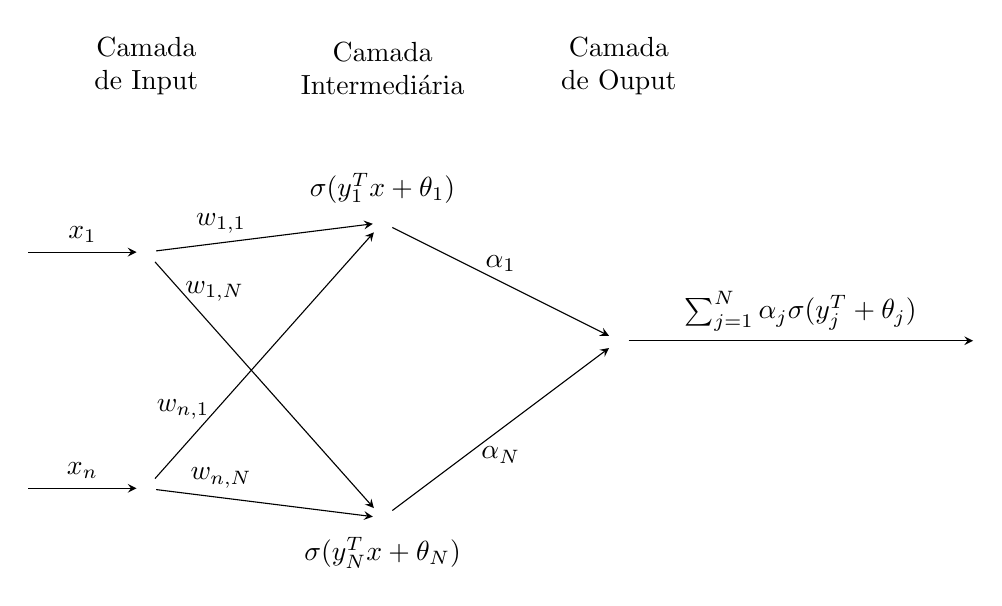
\begin{tikzpicture}[x=1.5cm, y=1.5cm, yshift=-1, >=stealth]

\foreach \m/\l [count=\y] in {1,missing,2}
  \node [every neuron/.try, neuron \m/.try] (input-\m) at (0,1.75-\y) {};

\foreach \m [count=\y] in {1,missing,2}
  \node [every neuron/.try, neuron \m/.try ] (hidden-\m) at (2,2.25-\y*1.25) {};

\foreach \m [count=\y] in {1}
  \node [every neuron/.try, neuron \m/.try ] (output-\m) at (4,1-\y) {};

\foreach \l [count=\i] in {1,n}
  \draw [<-] (input-\i) -- ++(-1,0)
    node [above, midway] {$x_\l$};

%% \foreach \l [count=\i] in {1,n}
%%   \node [above] at (hidden-\i.north) {$H_\l$};
\node [above] at (hidden-1.north) {\( \sigma (y_{ 1 }^{ T }x + \theta_{ 1 }) \)};
\node [below] at (hidden-2.south) {\( \sigma (y_{ N }^{ T }x + \theta_{ N }) \)};

\foreach \l [count=\i] in {1}
  \draw [->] (output-\i) -- ++(3,0)
    node [above, midway] {\( \sum_{ j=1 }^{ N } \alpha_{ j } \sigma (y_{ j }^{ T } + \theta_{ j }) \)};

%% \foreach \i in {1,...,2}
%%   \foreach \j in {1,...,2}
%%     \draw [->] (input-\i) -- (hidden-\j)
%%         node [above,pos=.2] {\( y_{ 1 }^{ (1) } \)};
\draw [->] (input-1) -- (hidden-1)
    node [above, pos=.3] {\( w_{ 1,1 } \)};
\draw [->] (input-2) -- (hidden-1)
    node [above, pos=.2, xshift=-2mm] {\( w_{ n,1 } \)};
\draw [->] (input-1) -- (hidden-2)
    node [above, pos=.2,xshift=2mm] {\( w_{ 1,N } \)};
\draw [->] (input-2) -- (hidden-2)
    node [above, pos=.3] {\( w_{ n,N } \)};

%% \foreach \i in {1,...,2}
%%   \foreach \j in {1}
%%     \draw [->] (hidden-\i) -- (output-\j);
\draw [->] (hidden-1) -- (output-1)
    node [above, midway] {\( \alpha_{ 1 } \)};
\draw [->] (hidden-2) -- (output-1)
    node [below, midway, yshift=-1mm] {\( \alpha_{ N } \)};

\foreach \l [count=\x from 0] in {de Input, Intermediária, de Ouput}
  \node [align=center, above] at (\x*2,2) {Camada \\ \l};

\end{tikzpicture}
    \end{center}
    \caption{Rede neural com apenas uma camada intermediária.
    Aqui temos \( x =
    \begin{bmatrix}
        x_{ 1 } & \cdots & x_{ n }
    \end{bmatrix}^{ T } \) e \( y_{ j }^{ T }x =
    \begin{bmatrix}
        w_{ 1,j } & \cdots & w_{ n,j }
    \end{bmatrix} \), o vetor dos pesos de cada nó intermediário.
    Na última camada ocorre apenas uma combinação linear.
    Repare que o output da rede é exatamente a expressão em (\ref{eq: neural_func}).}
    \label{fig: neural_net}
\end{figure}

Ou seja, o nosso objetivo nessa seção é estudar se podemos aproximar funções reais contínuas em \( \I^{ n } \) utilizando redes neurais com uma camada intermediária.
Essa é uma pergunta de extrema relevância, tanto teórica como prática pois, como apontado em \cite{lipmann}, redes neurais artificiais possuem diversas aplicações em campos voltados ao desenvolvimento de classificadores robustos, como a teoria de reconhecimento de fala e de imagens.
Saber que é possível realizar aproximações arbitrariamente boas utilizando redes neurais artificiais dá mais segurança e incentivo à pesquisa nessas áreas.

\subsection{O Teorema}

Denotaremos o espaço das funções reais contínuas em \( \I^{ n } \) por \( C(\I^{ n }) \) e o espaço das medidas de Borel finitas, com sinal e regulares em \( \I^{ n } \) por \( M(\I^{ n }) \).
Queremos entender sob quais condições as somas da forma \[
    G(x) = \sum_{ j=1 }^{ N } \alpha_{ j } \sigma(y_{ j }^{ T }x + \theta_{ j })
\]
são densas em \( C(\I^{ n }) \) com respeito à norma do supremo.
Faremos isso primeiro para uma classe mais geral de funções \( \sigma \) e depois mostraremos que as sigmoides pertencem a essa classe.

\begin{defn}
    Dizemos que \( \sigma \) é \emph{discriminatória} se, para uma medida \( \mu \in M(I^{ n }) \), termos \[
        \int_{ \I^{ n } } \sigma(y^{ T }x + \theta)  \ \mathrm{d}\mu = 0
    \]
    para todos \( y \in \R^{ n } \) e \( \theta \in \R \) implica em \( \mu = 0 \).
\end{defn}

\begin{teo}[Teorema da aproximação universal]
    Seja \( \sigma \) uma função contínua discriminatória qualquer.
    Então as somas finitas da forma \[
        G(x) = \sum_{ j=1 }^{ N } \alpha_{ j } \sigma(y_{ j }^{ T }x + \theta_{ j })
    \]
    são densas em \( C(\I^{ n }) \).
    Em outras palavras, dada qualquer \( f \in C(\I^{ n }) \) e \( \varepsilon > 0 \), existe uma soma, \( G(x) \), da forma acima, tal que \[
        \norm{ G - f }_{ \infty } < \varepsilon
    .\]
\end{teo}




\newpage

\printbibliography

\newpage

\appendix

% !TeX root = ./main.tex
\section{Elementos de Espaços Métricos}

Neste apêndice introduzimos o necessário para se compreender o Teorema de Baire, utilizado na demonstração do \( 13^{ \circ } \) problema de Hilbert.

\begin{defn}
    Dado um conjunto \( X \) qualquer, uma \emph{métrica} em \( X \) é uma função \( d : X \times X \to \R \) tal que:
    \begin{enumerate}[label=\roman*)]
        \item \( d(x, x) = 0 \);
        \item \( d(x, y) > 0 \) se \( x \neq y \);
        \item \( d(x, y) = d(y, x) \);
        \item \( d(x, z) \leq d(x, y) + d(y, z) \).
    \end{enumerate}
\end{defn}


\begin{defn}
    Um \emph{espaço métrico} é um par \( ( X, d ) \) onde \( X \) é um conjunto e \( d \) é uma métrica em \( X \).
\end{defn}

    Por vezes, onde não houver prejuízo ao entendimento do texto, utilizaremos apenas o nome do conjunto para nos referirmos ao espaço métrico por ele formado.

\begin{defn}
    Um suconjunto \( M \) de um espaço métrico \( X \) é dito \emph{limitado} se existe \( c \in \R \) tal que \( d(x, y) \leq c \) para todos \( x, y \in M \).
    Nesse caso, o definimimos o \emph{diâmetro} de \( M \), denotado por \( \diam M \), como \( \sup \left\{ d(x, y) \tq x, y \in M \right\} \).
    Se \( M \) é ilimitado, ou seja, para todo \( c > 0 \) existem \( x, y \in M \) com \( d(x, y) > c \), dizemos que \( \diam M = \infty \).
\end{defn}

%% \begin{exmp}[A reta]
%%     Um espaço métrico tradicional é o conjunto \( \R \) munido da métrica usual \( d : \R^2 \to \R \) dada por \( d(x, y) = \abs{ x-y }\).
%%     As propriedades i) a iv) resultam das propriedades básicas do valor absoluto de um número real.
%% \end{exmp}
%% 
%% \begin{exmp}[A métrica ``zero-um''] Todo conjunto \( X \) pode se tornar um espaço métrico se definirmos nele a métrica \( d \) dada por \( d(x, x) = 0 \) e \( d(x, y) = 1 \) se \( x \neq y \).
%% As propriedades necessárias são claramente verdadeiras.
%% \end{exmp}

\begin{defn}
    Dado um espaço métrico \( X \) e um ponto \( a \in X \), chamamos de \emph{bola aberta de raio r centrada em a} o conjunto \[
        B(a, r) \defeq \left\{ x \in X \tq d(x, a) < r \right\}
    .\]
\end{defn}

\begin{defn}
    Dado um espaço métrico \( X \) e um subconjunto \( Y \subset X \), chamamos de \emph{interior} de \( Y \), e denotamos por \( \intt Y \), o subconjunto de \( Y \) formado pelos elementos \( a \in Y \) tais que existe \( r > 0 \) satisfazendo \( B(a, r) \subset Y \).
\end{defn}

\begin{defn}
    Um subconjunto \( A \) de um espaço métrico \( X \) é dito \emph{aberto} se \( A = \intt A \).
\end{defn}

\begin{defn}
    Dado um subconjunto \( M \) de um espaço métrico \( X \), um ponto \( x \in X \) é dito \emph{aderente} a \( M \) se toda bola aberta centrada em \( x \) tiver interseção não-vazia com \( M \).
    Chamamos de \emph{fecho} de \( M \), e denotamos por \( \overline{M} \), o conjunto dos pontos de aderência de \( M \).
\end{defn}

\begin{defn}
    Um subconjunto \( F \) de um espaço métrico \( X \) é dito \emph{fechado} se \( F = \overline{F} \).
\end{defn}

\begin{defn}
    Dada uma sequência \( (x_{ n })_{ n \in \N } \) de elementos do espaço métrico \( X \), dizemos que \( (x_{ n })_{ n \in \N } \) \emph{converge} para \( L \in X \) se, dado \( \varepsilon > 0 \), existe \( n_{ 0 } \in \N \) tal que, para \( n \geq n_{ 0 } \), vale \( d(x_{ n }, L) < \varepsilon \).
    Se para todo \( L \in X \) é falso que \( \lim x_{ n } = L \), dizemos que \( ( x_{ n } ) \) é \emph{divergente}.
\end{defn}

\begin{defn}
    Uma sequência \( (x_{ n })_{ n \in \N } \) de elementos do espaço métrico \( X \) é dita \emph{de Cauchy} se, dado \( \varepsilon > 0 \), existe \( n_{ 0 } \in \N \) tal que, para \( n, m \geq n_{ 0 } \), vale \( d(x_{ n }, x_{ m }) < \varepsilon \).
    Equivalentemente, \( (x_{ n }) \) é de Cauchy se, para \( n \geq n_{ 0 } \), vale \( d(x_{ n }, x_{ n+p }) < \varepsilon \) para todo \( p \in \N \).
\end{defn}

\begin{prop}
    Toda sequência convergente \( (x_{ n })_{ n \in \N } \) no espaço métrico \( X \) é de Cauchy.
\end{prop}

\begin{proof}
    Seja \( L = \lim x_{ n } \).
    Dado \( \varepsilon > 0 \), tome \( n_{ 0 } \in \N \) de modo que, para \( n \geq n_{ 0 } \), valha \( d(x_{ n }, L) < \varepsilon/2 \).
    Então, se \( n, m \geq n_{ 0 } \) temos \[
        d(x_{ n }, x_{ m }) \leq d(x_{ n }, L) + d(x_{ m }, L) = \varepsilon/2 + \varepsilon/2 = \varepsilon
    .\qedhere\]
\end{proof}

\begin{exmp}
    Embora toda sequência convergente seja de Cauchy, é falso que dado um espaço métrico qualquer, toda sequência de Cauchy convirja para um ponto pertencente a ele.
    Por exemplo, considerando o conjunto \( \Q \) com a métrica \( d \) induzida pela métrica de \( \R \), temos que toda sequência de racionais convergindo para um irracional é de Cauchy, mas diverge em \( \Q \).
\end{exmp}

\begin{prop}
    Se \( ( x_{ n } )_{ n \in \N } \) em um espaço métrico \( X \) é de Cauchy e possui um valor de aderência (ou seja, existe uma subsequência convergente \( ( x_{ n_{ k } } ) \) de \( ( x_{ n } ) \)), então \( ( x_{ n } ) \) converge para esse valor de aderência.
\end{prop}

\begin{proof}
    Seja \( L \in X \) o limite da subsequência \( ( x_{ n_{ k } } ) \).
    Então, dado \( \varepsilon > 0 \) conseguimos obter \( k_{ 0 } \in \N \) tal que, se \( k > k_{ 0 } \), então \( d(x_{ n_{ k } }, L) < \varepsilon/2 \).
    Também conseguimos \( n_{ 0 } \in \N \) tal que, se \( n, m \geq n_{ 0 } \) então \( d(x_{ n }, x_{ m }) < \varepsilon/2 \).
    Tome \( \ell > \max \left\{ n_{ 0 }, k_{ 0 } \right\} \).
    Então claramente \( n_{ \ell } \geq \ell \) e, com isso, \[
        d(x_{ \ell }, L) \leq d(x_{ \ell }, x_{ n_{ \ell } }) + d(x_{ n_{ \ell } }, L) < \varepsilon/2 + \varepsilon/2 = \varepsilon
    .\qedhere\]
\end{proof}


\begin{defn}
    Um espaço métrico \( X \) é dito \emph{completo} se toda sequência de Cauchy em \( X \) converge para um elemento de \( X \).
\end{defn}



\begin{prop}
    \label{prop: fechados_encaixados}
    Um espaço métrico \( X \) é completo se, e somente se, dada uma sequência decrescente \( F_{ 1 } \supset F_{ 2 } \supset \cdots \) de conjuntos não-vazios fechados em \( X \), tais que \( \lim \diam F_{ n } = 0 \), existe \( a \in X \) com \[
        \left\{ a \right\} = \bigcap_{ n=1 }^{ \infty } F_{ i }
    .\]
\end{prop}

\begin{proof}
    Suponha que \( X \) seja completo e considere \( ( F_{ n } )_{ n \in \N } \) como no enunciado do teorema.
    Para cada conjunto \( F_{ n } \), escolha \( x_{ n } \in F_{ n } \), formando uma sequência \( ( x_{ n } )_{ n \in \N } \) de Cauchy.
    De fato, como \( \lim \diam F_{ n } = 0 \), dado \( \varepsilon > 0 \) existe \( n_{ 0 } \in \N \) tal que para \( n \geq n_{ 0 } \), temos \( d(x, y) < \varepsilon \) para todos \( x, y \in F_{ n } \).
    De \( F_{ 1 } \supset F_{ 2 } \supset \cdots \) concluímos que \( n, m > n_{ 0 } \) implicam \( x_{ n }, x_{ m } \in F_{ n_{ 0 } } \) o que implica \( d(x_{ n }, x_{ m }) < \varepsilon \).

    Da completude de \( X \) concluímos que existe \( a = \lim x_{ n } \).
    Como todos \( F_{ n } \) são fechados e, para \( m \geq n \) temos \( x_{ m } \in F_{ n } \), conclui-se que \( a \in F_{ n } \) para todo \( n \in \N \), ou seja, \[
        a \in \bigcap_{ n=1 }^{ \infty } F_{ n }
    .\]
    Suponha, agora, que \( X \) seja um espaço métrico no qual toda sequência de fechados como a do enunciado convirja.
    Seja \( ( x_{ n } )_{ n \in \N } \) uma sequência de Cauchy em \( X \).
    Defina, para cada \( n \in \N \), o conjunto \( F_{ n } = \left\{ x_{ n }, x_{ n+1 }, \dots \right\} \).
    Então \( ( \overline{F_{ n }} )_{ n \in \N } \) é uma sequência decrescente de conjuntos fechados tais que \( \lim \diam \overline{F_{ n }} = \lim \diam F_{ n } = 0 \).
    Por hipótese, existe \( a \in \bigcap \overline{F_{ n }} \).
    Como \( a \) é limite de sequência de pontos de \( F_{ k } \) para todo \( k \in \N \), para cada \( k \) podemos escolher \( a_{ n_{ k } } \in F_{ k } \) de modo que \( d(a, a_{ n_{ k } }) < 1/k \) e, assim,  \( \lim a_{ n_{ k } } = a \).
    Claramente \( n_{ k } > k \) para todo \( k \in \N \), portanto, passando a uma subsequência se necessário, \( a_{ n_{ k } } \) é subsequência de \( (x_{ n }) \) o que implica, como \( (x_{ n }) \) é de Cauchy, \( \lim x_{ n } = a \).
\end{proof}

\begin{teo}[Teorema da Categoria de Baire]
    Se \( X \) é um espaço métrico completo e \( A_{ 1 }, A_{ 2 }, \dots \) são abertos densos em \( X \), então \[
        A = \bigcap_{ i=1 }^{ \infty } A_{ i }
    \]
    é denso em \( X \).
\end{teo}

\begin{proof}
    Devemos mostrar que dado \( V \) um conjunto aberto em \( X \), temos \( A \cap V \neq \emptyset \).
    Nossa estratégia será construir uma sequência decrescente \( F_{ 1 } \supset F_{ 2 } \supset \cdots \) de conjuntos fechados não-vazios tais que \( \lim \diam F_{ n } = 0 \) e, para todo \( n \in \N \), \( F_{ n } \subset A_{ n } \cap V \).
    Então, pela Proposição \ref{prop: fechados_encaixados}, o ponto \( x \) que satisfaz \( \left\{ x \right\} = \bigcap F_{ n } \) é tal que \( x \in V \) e \( x \in F_{ n } \subset A_{ n } \) para todo \( n \), ou seja, \( x \in A \) e, portanto, \( x \in A \cap V \).

    Começamos obeservando que, como \( A_{ 1 } \) é denso, \( A_{ 1 } \cap V \) é um conjunto aberto não-vazio.
    Logo, existe \( B_{ 1 } \) bola aberta não-vazia de raio menor que \( 1 \), tal que \( \overline{B_{ 1 }} \subset A_{ 1 } \cap V \).
    Suponha, agora, definidos \( B_{ 1 }, \dots, B_{ n } \) de forma que, para todo \( 1 < k \leq n \), \( B_{ k } \) é uma bola aberta não-vazia de raio menor que \( 1/k \) tal que \( \overline{B_{ k }} \subset V \cap A_{ k } \cap B_{ k-1 } \).
    Novamente, como \( A_{ n+1 } \) é denso, \( A_{ n+1 } \cap B_{ n } \) é um conjunto aberto não vazio.
    Logo, definimos \( B_{ n+1 } \) como uma bola aberta não-vazia contida em \( A_{ n+1 } \cap B_{ n } \), de raio menor que \( 1/( n+1 ) \) tal que \( \overline{B_{ n+1 }} \subset A_{ n+1 } \cap B_{ n } \subset A_{ n+1 } \cap V \ \).

    Com isso, obtemos uma sequência decrescente \( B_{ 1 } \supset \cdots \supset B_{ n } \supset \cdots \) de bolas abertas não-vazias, com o raio de \( B_{ n } \) menor que \( 1/n \), cujos fechos \( \overline{B_{ 1 }} \supset \cdots \supset \overline{B_{ n }} \supset \cdots \) formam uma sequência decrescente de conjuntos fechados não-vazios, com \( \diam \overline{B_{ n }} \leq 1/n \) e \( \overline{B_{ n }} \subset A_{ n } \cap V \) para todo \( n \in \N \), o que, como apontado anteriormente, termina a prova.
\end{proof}

Terminaremos essa seção com a definição de função contínua, que será usada posteriormente.

\begin{defn}
    Dados espaços métricos \( (X, d_{ X }) \) e \( (Y, d_{ Y }) \), uma função \( f : X \to Y \) é dita \emph{contínua} em \( a \in X \) se, para todo \( \varepsilon > 0 \), existe \( \delta > 0 \) tal que, se \( d_{ X }(x, a) < \delta \), então \( d_{ Y }(f(x), f(a)) < \varepsilon \).
\end{defn}

% !TeX root = ./main.tex

\section{Elementos de Análise Funcional}
\label{app: func anal}

Aqui apresentaremos noções elementares que mesclam conceitos de Análise e de Álgebra Linear.

\begin{defn}
    Dado um espaço vetorial \( V \) sobre um corpo \( \K \), uma \emph{norma} em \( V \) é uma função \( \norm{ \cdot } : V \to [0, +\infty) \) tal que
    \begin{enumerate}[label=\roman*)]
        \item \( \norm{ v } = 0 \) se, e somente se \( v = 0 \) (normas são \emph{positivas definidas});
        \item \( \norm{ \alpha v } = \abs{ \alpha } \norm{ v } \) para todo \( v \in V \) e \( \alpha \in \K \) (\emph{homogeneidade absoluta});
        \item \( \norm{ v + w } \leq \norm{ v } + \norm{ w } \) para todos \( v, w \in V \) (\emph{desigualdade triangular}).
    \end{enumerate}
\end{defn}
Uma função que cumpre as propriedades \emph{ii} e \emph{iii} acima é denominada uma \emph{semi-norma}.
Um espaço vetorial junto de sua norma e denominado um \emph{espaço vetorial normado}.
A menos de onde houver ambiguidade, utilizaremos o mesmo símbolo \( \norm{ \cdot } \) para nos referir a normas de qualquer espaço vetorial normado.
O vetor dentro do símbolo deixará claro a norma de qual espaço está sendo utilizada.

É interessante perceber que todo espaço vetorial normado é um espaço métrico, quando se introduz nele a métrica induzida pela norma: \( (v, w) \mapsto \norm{ v - w } \).
As propriedades de uma métrica são facilmente verificadas.

\begin{defn}
    Uma transformação linear \( T : V \to W \) entre dois espaços vetoriais normados é dita \emph{limitada} se existe \( C \in [0, +\infty) \) tal que \( \norm{ Tv } \leq C \norm{ v } \) para todo \( v \in V \).
\end{defn}
Essa definição naturalmente é diferente da definição usual de função limitada, pois, como \( T(\lambda v) = \lambda (Tv) \), impossível termos \( \norm{ Tv } \leq C \) para todo \( v \in V \) se \( T \) é não nula.

O próximo teorema ilustra a utilidade dessa definição de transformação limitada.

\begin{teo}
    Seja \( T : V \to W \) uma transformação linear entre espaços vetoriais normados.
    As seguintes afirmativas são equivalentes:
    \begin{enumerate}[label=\roman*)]
        \item \( T \) é contínua;
        \item \( T \) é contínua em \( 0 \);
        \item \( T \) é limitada.
    \end{enumerate}
\end{teo}
\begin{proof}
    A implição de \emph{i} para \emph{ii} é óbvia.
    Suponha, agora, que \( T \) é contínua em \( 0 \).
    Tomando \( \varepsilon = 1 \), conseguimos \( \delta > 0 \) tal que se \( \norm{ v } \leq \delta \), então \( \norm{ Tv } < 1 \).
    Agora, dado \( v \in V \), \( v \neq 0 \), tome o vetor \( v' \defeq \delta v / \norm{ v } \).
    Claramente temos \( \norm{ v' } = \delta \), ou seja, \( \norm{ Tv' } < 1 \), o que implica \( \norm{ Tv } < \delta^{ -1 } \norm{ v } \).
    Logo, tomando \( C = \delta^{ -1 } \), \( T \) é limitada.
    Por fim, se \( T \) é limitada, dados \( a \in V \) e \( \varepsilon \), tome \( \delta < \varepsilon/C \).
    Com isso se \( \norm{ x - a } < \delta \) temos: \[
        \norm{ Tx - Ta } = \norm{ T(x - a) } \leq C \norm{ x - a } < C \cdot \varepsilon/C = \varepsilon
    .\]
    Portanto, \( T \) é contínua.
\end{proof}

Denotamos pro \( L(V, W) \) o conjunto das transformações lineares limitadas de \( V \) em \( W \).
Esse conjunto, com as operações usuais de adição e multiplicação por escalar, é um espaço vetorial.
Podemos, ainda, definir nele uma norma, dada por
\begin{align}
    \norm{ T } &\defeq \sup \left\{ \frac{ \norm{ Tv } }{ \norm{ v } } : v \in V \backslash \left\{ 0 \right\} \right\} \label{ali: first} \\
    &= \sup \left\{ \norm{ Tv } : v \in V, \norm{ v } = 1 \right\} \label{ali: sec} \\
    &= \inf \left\{ C : \norm{ Tv } \leq C \norm{ v } \text{ para todo } v \in V \right\}
    \label{ali: third}
.\end{align}
Claramente os dois primeiros conjuntos são iguais, logo seus supremos também o são.
Para ver que vale (\ref{ali: third}), perceba que, por (\ref{ali: first}), temos \( \norm{ Tv } \leq \norm{ T } \norm{ v } \) para todo \( v \in V \).
Portanto, sendo \( A \) o conjunto em (\ref{ali: third}), temos \( \norm{ T } \in A \), ou seja, \( \inf A \leq \norm{ T } \).
Além disso, dado \( C \in A \), temos \( C \geq \norm{ Tv } / \norm{ v } \) para todo \( v \in V - \left\{ 0 \right\} \).
Logo, \( \norm{ T } \leq C \) e, com isso, \( \norm{ T } \leq \inf A \).
Sendo assim, vale (\ref{ali: third}).
As propriedades i), ii) e iii) decorrem diretamente das propriedades das normas de \( V \) e \( W \) e são facilmente verificadas.
Sempre trataremos o conjunto \( L(V, W) \) como um espaço vetorial normado munido dessa norma, a qual é denominada \emph{norma de operador}. 
No caso especial em que \( W = \K \),
o espaço \( L(V, \K) \) é denominado \emph{espaço dual} de \( V \) e é denotado por \( V^{ * } \).
Os elementos de \( V^{ * } \) são denominados \emph{funcionais lineares}.

\begin{defn}
    Um \emph{produto interno} no espaço vetorial \( V \) é um funcional \( (v, w) \mapsto \dotprod{v,w} \), de \( V \times V \) em \( \K \), de modo que, para todos \( u, v, w \in V \) e \( \alpha \in \K \) valha
    \begin{enumerate}[label=\roman*)]
        \item \( \dotprod{\alpha v + u, w} = \bar{\alpha} \dotprod{v, w} + \dotprod{u, w} \);
        \item \( \dotprod{v, w} = \overline{\dotprod{v,w}} \);
        \item \( \dotprod{v, v} \geq \) e \( \dotprod{v, v} = 0 \) se, e somente se, \( v = 0 \).
    \end{enumerate}
    O par \( (V, \dotprod{\cdot,\cdot}) \) é chamado, então, de \emph{espaço com produto interno} ou \emph{espaço pré-Hilbertiano}.
\end{defn}
Como de costume, \( \bar{\alpha} \) denota o complexo conjugado de \( \alpha \).
Em um espaço vetorial com produto interno, a menos que se dia o contrário, tem-se \( \norm{ v } = \sqrt{ \dotprod{v,v} } \).
De fato essa função define uma norma em \( V \), como será mostrado a seguir.
Antes, porém, devemos estabelecer um resultado fundamental em espaços com produto interno.
\begin{teo}[Desigualdade de Cauchy-Schwarz]
    Em um espaço com produto interno \( (V, \dotprod{\cdot,\cdot}) \), tem-se \[
        \abs{ \dotprod{v, w} } \leq \norm{ v } \norm{ w }
    \]
    para todos \( v, w \in V \), com a igualdade ocorrendo se, e somente se, \( v = \lambda w \).
\end{teo}
\begin{proof}
    Se \( \dotprod{v, w} = 0 \), a igualdade é imediata.
    Caso contrário, então \( w \neq 0 \) e, para \( \lambda \in \K \) tem-se \[
        0 \leq \dotprod{v - \lambda w, v - \lambda w} = \norm{ v }^2 -\lambda \dotprod{v, w} -\bar{\lambda} \dotprod{w, v} + \abs{ \lambda }^2 \norm{ w }^2
    .\]
    tomando \( \lambda = \dotprod{w, v}/\norm{ w }^2 \) vem \[
        0 \leq \norm{ v }^2 - \abs{ \dotprod{v, w} }^2/ \norm{ w }^2
    ,\]
    o que implica \[
        \abs{ \dotprod{v, w} }^2 \leq \norm{ v }^2 \norm{ w }^2
    ,\]
    de onde o resultado se segue.
    Naturalmente a igualdade ocorre se e somente se existe \( \lambda \) tal que \( \dotprod{v - \lambda w, v - \lambda w} = 0 \), ou seja, \( v = \lambda w \).
\end{proof}

É fácil ver que as duas primeiras propriedades da norma são satisfeitas por \( \norm{ \cdot } \) como definida anteriormente.
Para verficar a desigualdade triangular perceba que
\begin{align*}
    \norm{ v + w }^2
    &= \norm{ v }^2 + 2 \Re \dotprod{v, w} + \norm{ w }^2 \\
    &\leq \norm{ v }^2 + 2 \abs{ \dotprod{v, w} } + \norm{ w }^2 \\
    &\leq \norm{ v }^2 + 2 \norm{ v } \norm{ w } + \norm{ w }^2 \\
    &= ( \norm{ v } + \norm{ w } )^2
.\end{align*}
Portanto, \( \norm{ \cdot } \) de fato é uma norma, denominada \emph{norma induzida pelo produto interno}.

\begin{defn}
    Um \emph{espaço de Hilbert} é um espaço com produto interno completo com relação à norma induzida pelo produto interno.
\end{defn}

\end{document}